%%% The main file. It contains definitions of basic parameters and includes all other parts.

%% Settings for single-side (simplex) printing
% Margins: left 40mm, right 25mm, top and bottom 25mm
% (but beware, LaTeX adds 1in implicitly)
\documentclass[12pt,a4paper]{report}
\setlength\textwidth{145mm}
\setlength\textheight{247mm}
\setlength\oddsidemargin{15mm}
\setlength\evensidemargin{15mm}
\setlength\topmargin{0mm}
\setlength\headsep{0mm}
\setlength\headheight{0mm}
% \openright makes the following text appear on a right-hand page
\let\openright=\clearpage

%% Settings for two-sided (duplex) printing
% \documentclass[12pt,a4paper,twoside,openright]{report}
% \setlength\textwidth{145mm}
% \setlength\textheight{247mm}
% \setlength\oddsidemargin{14.2mm}
% \setlength\evensidemargin{0mm}
% \setlength\topmargin{0mm}
% \setlength\headsep{0mm}
% \setlength\headheight{0mm}
% \let\openright=\cleardoublepage

%% Generate PDF/A-2u
\usepackage[a-2u]{pdfx}

%% Character encoding: usually latin2, cp1250 or utf8:
\usepackage[utf8]{inputenc}

%% Prefer Latin Modern fonts
\usepackage{lmodern}

%% Further useful packages (included in most LaTeX distributions)
\usepackage{amsmath}        % extensions for typesetting of math
\usepackage{amsfonts}       % math fonts
\usepackage{amsthm}         % theorems, definitions, etc.
\usepackage{amssymb}
\usepackage{bbding}         % various symbols (squares, asterisks, scissors, ...)
\usepackage{bm}             % boldface symbols (\bm)
\usepackage{graphicx}       % embedding of pictures
\usepackage{fancyvrb}       % improved verbatim environment
\usepackage{natbib}         % citation style AUTHOR (YEAR), or AUTHOR [NUMBER]
\usepackage[nottoc]{tocbibind} % makes sure that bibliography and the lists
			    % of figures/tables are included in the table
			    % of contents
\usepackage{dcolumn}        % improved alignment of table columns
\usepackage{booktabs}       % improved horizontal lines in tables
\usepackage{paralist}       % improved enumerate and itemize
\usepackage{xcolor}         % typesetting in color
\usepackage{tabularx}
\usepackage[toc,nogroupskip,nopostdot]{glossaries}
\usepackage{todonotes}
\usepackage{enumitem}

\usepackage{caption}
\usepackage{subcaption}
\usepackage{siunitx}

\usepackage{footnotehyper} % TODO


\setlist[enumerate]{topsep=0pt,itemsep=-1ex,partopsep=1ex,parsep=1ex}
%\usepackage{svg}

\usepackage{xcolor} % TODO TODO TODO
\usepackage{gensymb}
\usepackage{mathtools}
\usepackage{caption}
\usepackage[ruled,vlined]{algorithm2e}

\makenoidxglossaries
\loadglsentries{glossary}
%
\newglossaryentry{VL}
{
    name=Videolytics,
    description={Encapsulating system this work is module of}
}

\newglossaryentry{det}
{
    name=detection,
    %text=detection,
    description={image of a detected object within a frame with spatial metadata},
    first=\emph{detection},
    firstplural=\emph{detections},
}

\newglossaryentry{iden}
{
    name=identity,
    %text=identity,
    plural=identities,
    description={set of detections displaying the same object}
    first=\emph{identity},
    firstplural=\emph{identities},
}

\newglossaryentry{ses}
{
    name=session,
    %text=session,
    description={pair of set of detections and its associated ``golden'' partitioning},
    first=\emph{session},
    firstplural=\emph{sessions},
}

\newacronym{ml}{ML}{machine learning}
\newacronym{api}{API}{application programming interface}
\newacronym{mle}{MLE}{maximum likelihood estimator}
\newacronym{mse}{MSE}{mean square error}

\newglossaryentry{nn}
{
    name={neural network},
    description={popular machine learning model},
    plural={neural networks},
    first=\emph{neural network},
    firstplural=\emph{neural networks},
}

\newacronym{em}{EM}{estimation maximisation}

\newacronym{tp}{TP}{true positive}
\newacronym{tn}{TN}{true negative}
\newacronym{fp}{FP}{false positive}
\newacronym{fn}{FN}{false negative}
\newacronym{tpr}{TPR}{true positive rate}
\newacronym{fpr}{FPR}{false positive rate}
\newacronym{roc}{ROC}{receiver operating characteristic}

%%% Basic information on the thesis

% Thesis title in English (exactly as in the formal assignment)
\def\ThesisTitle{Re-identification of Objects in Video Stream using Data Analytics}

% Author of the thesis
\def\ThesisAuthor{Dominik Smrž}

% Year when the thesis is submitted
\def\YearSubmitted{2021}

% Name of the department or institute, where the work was officially assigned
% (according to the Organizational Structure of MFF UK in English,
% or a full name of a department outside MFF)
\def\Department{Department of Software Engineering}

% Is it a department (katedra), or an institute (ústav)?
\def\DeptType{Department}

% Thesis supervisor: name, surname and titles
\def\Supervisor{prof. RNDr. Tomáš Skopal, Ph.D.}

% Supervisor's department (again according to Organizational structure of MFF)
\def\SupervisorsDepartment{Department of Software Engineering}

% Study programme and specialization
\def\StudyProgramme{Computer Science}
\def\StudyBranch{Artificial Intelligence}

% An optional dedication: you can thank whomever you wish (your supervisor,
% consultant, a person who lent the software, etc.)
\def\Dedication{%
Dedication.
}

% Abstract (recommended length around 80-200 words; this is not a copy of your thesis assignment!)
\def\Abstract{%
Abstract.
}

% 3 to 5 keywords (recommended), each enclosed in curly braces
\def\Keywords{%
{key} {words}
}

%% The hyperref package for clickable links in PDF and also for storing
%% metadata to PDF (including the table of contents).
%% Most settings are pre-set by the pdfx package.
\hypersetup{hidelinks}
\hypersetup{unicode}
\hypersetup{breaklinks=true}

% Definitions of macros (see description inside)
%%% This file contains definitions of various useful macros and environments %%%
%%% Please add more macros here instead of cluttering other files with them. %%%

%%% Minor tweaks of style

% These macros employ a little dirty trick to convince LaTeX to typeset
% chapter headings sanely, without lots of empty space above them.
% Feel free to ignore.
\makeatletter
\def\@makechapterhead#1{
  {\parindent \z@ \raggedright \normalfont
   \Huge\bfseries \thechapter. #1
   \par\nobreak
   \vskip 20\p@
}}
\def\@makeschapterhead#1{
  {\parindent \z@ \raggedright \normalfont
   \Huge\bfseries #1
   \par\nobreak
   \vskip 20\p@
}}
\makeatother

% This macro defines a chapter, which is not numbered, but is included
% in the table of contents.
\def\chapwithtoc#1{
\chapter*{#1}
\addcontentsline{toc}{chapter}{#1}
}

% Draw black "slugs" whenever a line overflows, so that we can spot it easily.
\overfullrule=1mm

%%% Macros for definitions, theorems, claims, examples, ... (requires amsthm package)

\theoremstyle{plain}
\newtheorem{thm}{Theorem}
\newtheorem{lemma}[thm]{Lemma}
\newtheorem{claim}[thm]{Claim}

\theoremstyle{plain}
\newtheorem{defn}{Definition}

\theoremstyle{remark}
\newtheorem*{cor}{Corollary}
\newtheorem*{rem}{Remark}
\newtheorem*{example}{Example}

\newcommand{\defnautorefname}{definition}

%%% An environment for proofs

\newenvironment{myproof}{
  \par\medskip\noindent
  \textit{Proof}.
}{
\newline
\rightline{$\qedsymbol$}
}

%%% An environment for typesetting of program code and input/output
%%% of programs. (Requires the fancyvrb package -- fancy verbatim.)

\DefineVerbatimEnvironment{code}{Verbatim}{fontsize=\small, frame=single}

%%% The field of all real and natural numbers
\newcommand{\R}{\mathbb{R}}
\newcommand{\N}{\mathbb{N}}
\newcommand{\Pt}[1]{\mathcal{P}\left(#1\right)}
\newcommand{\reid}{re-identification}
\newcommand{\Reid}{Re-identification}

%%% Useful operators for statistics and probability
\DeclareMathOperator{\pr}{\textsf{P}}
\DeclareMathOperator{\E}{\textsf{E}\,}
\DeclareMathOperator{\var}{\textrm{var}}
\DeclareMathOperator{\sd}{\textrm{sd}}

%%% Transposition of a vector/matrix
\newcommand{\T}[1]{#1^\top}

%%% Various math goodies
\newcommand{\goto}{\rightarrow}
\newcommand{\gotop}{\stackrel{P}{\longrightarrow}}
\newcommand{\maon}[1]{o(n^{#1})}
\newcommand{\abs}[1]{\left|{#1}\right|}
\newcommand{\dint}{\int_0^\tau\!\!\int_0^\tau}
\newcommand{\isqr}[1]{\frac{1}{\sqrt{#1}}}

%%% Various table goodies
\newcommand{\pulrad}[1]{\raisebox{1.5ex}[0pt]{#1}}
\newcommand{\mc}[1]{\multicolumn{1}{c}{#1}}

\newcommand{\algautorefname}{Algorithm}
\newcommand{\clmautorefname}{Claim}

\DeclarePairedDelimiter\ceil{\lceil}{\rceil}
\DeclarePairedDelimiter\floor{\lfloor}{\rfloor}

\let\origitemize\itemize
\renewcommand\itemize{\origitemize\addtolength{\itemsep}{-6pt}}

% Title page and various mandatory informational pages
\begin{document}
%%% Title page of the thesis and other mandatory pages

%%% Title page of the thesis

\pagestyle{empty}
\hypersetup{pageanchor=false}
\begin{center}

\centerline{\mbox{
\includegraphics[width=166mm]{img/logo-en.pdf}}}

\vspace{-8mm}
\vfill

{\bf\Large MASTER THESIS}

\vfill

{\LARGE\ThesisAuthor}

\vspace{15mm}

{\LARGE\bfseries\ThesisTitle}

\vfill

\Department

\vfill

{
\centerline{\vbox{\halign{\hbox to 0.45\hsize{\hfil #}&\hskip 0.5em\parbox[t]{0.45\hsize}{\raggedright #}\cr
Supervisor of the master thesis:&\Supervisor \cr
\noalign{\vspace{2mm}}
Study programme:&\StudyProgramme \cr
\noalign{\vspace{2mm}}
Study branch:&\StudyBranch \cr
}}}}

\vfill

% Zde doplňte rok
Prague \YearSubmitted

\end{center}

\newpage

%%% Here should be a bound sheet included -- a signed copy of the "master
%%% thesis assignment". This assignment is NOT a part of the electronic
%%% version of the thesis. DO NOT SCAN.

%%% A page with a solemn declaration to the master thesis

\openright
\hypersetup{pageanchor=true}
\pagestyle{plain}
\pagenumbering{roman}
\vglue 0pt plus 1fill

\noindent
I declare that I carried out this master thesis independently, and only with the cited
sources, literature and other professional sources. It has not been used to obtain another
or the same degree.

\medskip\noindent
I understand that my work relates to the rights and obligations under the Act No.~121/2000 Sb.,
the Copyright Act, as amended, in particular the fact that the Charles
University has the right to conclude a license agreement on the use of this
work as a school work pursuant to Section 60 subsection 1 of the Copyright~Act.

\vspace{10mm}

\hbox{\hbox to 0.5\hsize{%
In \hbox to 6em{\dotfill} date \hbox to 6em{\dotfill}
\hss}\hbox to 0.5\hsize{\dotfill\quad}}
\smallskip
\hbox{\hbox to 0.5\hsize{}\hbox to 0.5\hsize{\hfil Author's signature\hfil}}

\vspace{20mm}
\newpage

%%% Dedication

\openright

\noindent
\Dedication

\newpage

%%% Mandatory information page of the thesis

\openright

\vbox to 0.5\vsize{
\setlength\parindent{0mm}
\setlength\parskip{5mm}

Title:
\ThesisTitle

Author:
\ThesisAuthor

\DeptType:
\Department

Supervisor:
\Supervisor, \SupervisorsDepartment

Abstract:
\Abstract

Keywords:
\Keywords

\vss}

\newpage

\openright
\pagestyle{plain}
\pagenumbering{arabic}
\setcounter{page}{1}


%%% A page with automatically generated table of contents of the master thesis

\tableofcontents

%%% Each chapter is kept in a separate file
\chapter*{Introduction}
\addcontentsline{toc}{chapter}{Introduction}

\label{ch:intro}

Increasing usage of surveillance cameras brought many opportunities for further data exploration. Aside from the obvious usage in a security, such a vast amount of data allows for traffic monitoring and statistical processing of peoples' behavioral patterns. Obtained data can then be in turn used for improved urban planning or marketing purposes.

However, to explore any long-term processes such as the movement of people, we need to match the same individual across different points in time or even different cameras. This problem is widely referred to as \reid{} task in the literature, and this thesis mainly focuses on this task.

Many different approaches were taken to solve the \reid{} problem. Some of them process mainly spatial information (\cite{hu2006principal}). However, with the advancement in machine learning more and more approaches focus solely on the visual side of the problem. We often see a general workflow, where a deep neural network is used to extract the visual information from the image of a tracked object. The extracted information is then used for the \reid{} (\cite{ding2015deep} or \cite{cheng2016person}).

In this work, we offer a \reid{} pipeline that combines the spatial and temporal information with the descriptors extracted from the images. We design our work as a module for \gls{VL} by \cite{videolytics} -- an analytical system for video surveillance. In our approach, we split the task into two separate stages.

The first stage focuses on encoding the visual information from the stream into a more compact representation. We explore a few options for a suitable representation. One set of approaches is based on the color distribution in the images in the form of color histograms. The other representation we test is obtained deep neural networks. We evaluate and design various architectures based on the recent advancement in image processing.

In the second stage, we incorporate the information about the position of an object. We mainly use this information to match the objects in consecutive frames, where the physical position does not vary too much. We use this matching to a lower number of comparisons based on the visual information.

We conduct a thorough evaluation of our approaches. To express the quality of the model we focus on the question whether two given datapoints correspond to the same object. We then evaluate how often the proposed model produces the correct answer.

Aside from the theoretical presentation of our approach to the \reid{} task we implement an entire framework encapsulating the issue. We offer the complete pipeline: Querying the detected objects from the database, processing and re-identifying the objects, and storing the results back to the database. The implementation allows for easy testing of other approaches for the \reid{} task on the available data. We also implement an annotation tool that can also be used for in-depth analysis of any given re-identification algorithm. We used this tool to produce the manual annotations used for the evaluation of proposed approaches.


% Aside from the actual re-identification pipeline, we present an entire framework encapsulating the issue. We implement an easy-to-use pipeline that can be used for testing other approaches to the problem. We also implement an annotation tool that can also be used for in-depth analysis of any given re-identification algorithm. We used this tool to produce the manual annotations used for the evaluation of proposed approaches.

\subsection*{Thesis Structure}

The work in this thesis is organized as follows:

Firstly, we summarize the general theoretical background. In \autoref{ch:preliminaries} we introduce the notation we use. We also present the basics of machine learning and neural networks in particular. In \autoref{ch:related_work} we review the recent advancement in the area. Aside from work related to the re-identification task itself, we also review neural network architectures for image processing in general.

In the remaining chapters, we present our contribution. In \autoref{ch:workflow} we formally define our task. We also show the general workflow of our work in the context of \gls{VL}. The chapters \ref{ch:features} and \ref{ch:iden_construction} describe the actual algorithm for re-identification. In \autoref{ch:features} we focus on how we extract useful visual information from the images of detected objects. In \autoref{ch:iden_construction} we then combine this information with spatial and temporal information to produce final \reid{}. The proposed model is thoroughly evaluated in \autoref{ch:evaluation}. In the \autoref{ch:implementation} we discuss the underlying implementation. We describe the architecture and technical aspects of the attached source code.
\chapter{Preliminaries}

%123456789 123456789 123456789 123456789 123456789 123456789 123456789 123456789

In this chapter, we provide an overview of the elementary concepts we use in the thesis. We start by introducing the basic notation we shall
use thorough out the work. Then we show the concept of distances and
metric spaces. We finish the chapter by describing the basics of
neural networks and related concepts.

\section{Notation}

We briefly summarize the notation we use. We use standard notation for number systems: $\mathbb{N}$ for natural numbers (including zero), $\mathbb{R}$ for real numbers, $\mathbb{R}^+$ for positive real numbers, and $\mathbb{R}^+_0$ for non-negative real numbers.

We often work with vectors, and we shall write them as $\vec{a}$. In order to refer to $i$-th element of a vector $\vec{a}$ we shall write $a_i$. Similarly, in the case of matrix $A$, we shall refer to a specific element in $i$-th row and $j$-th column as $A_{i,j}$.

Finally, we shall use the term \emph{tensor} as a generalization of vectors and matrices. We shall use the following recursive definition:

\begin{defn}
0-dimensional tensor is a single number. n-dimensional ($n > 0$) vector of sizes
$(s_1, s_2, \ldots, s_n)$ is an ordered set of $s_1$ $(n-1)$-dimensional
tensors of sizes $(s_2, s_3, \ldots, s_n)$.
\end{defn}

As we can see, a 1-dimensional tensor is a vector, and a 2-dimensional tensor is a matrix. Similarly, we shall refer to specific element of tensor $a$ using subscripts ($a_{i,j,k}$).

\section{Distance and Metric Spaces}
\label{sec:distances}

In this work, we often need to express the similarity between two data points (usually images or their representation). To provide a precise mathematical background for such similarity, we use the concept of metric spaces introduced by \cite{metric} and named by \cite{metricname}. We further differentiate between metrics (and metric spaces) and distances (and distance spaces). We use definitions per \cite{deza2009encyclopedia}.

\begin{defn}
Metric space $(\mathcal{F}, \delta)$ is a pair of set $\mathcal{F}$ and
corresponding distance function
$\delta : \mathcal{F} \times \mathcal{F} \goto \mathbb{R}_0^+$ such that
following axioms hold:
\begin{itemize}
    \item $\delta(x, y) = 0 \Leftrightarrow x = y$ (Coincidence axiom)
    \item $\delta(x, y) = \delta(y, x)$ (Axiom of symmetry)
    \item $\delta(x, y) \leq \delta(x, z) + \delta(z, y)$ (Triangle inequality)
\end{itemize}
\end{defn}%

However, as these axioms prove to be too restrictive in some cases, we also use the concept of distance space:
\begin{defn}
Distance space $(\mathcal{F}, \delta)$ is a pair of set $\mathcal{F}$ and
corresponding distance function $\delta : \mathcal{F} \times \mathcal{F} \goto \mathbb{R}_0^+$ such that
following axioms hold:
\begin{itemize}
    \item $\delta(x, y) = \delta(y, x)$
    \item $\delta(x, x) = 0$
\end{itemize}
\end{defn}%
It is easy to see that each metric space is also a distance space.

\subsection{Used Distances and Metrics}

\label{ssec:used_distances}

In this subsection, we briefly introduce the specific metrics and distances we use in this thesis.

\begin{defn}
Euclidean space is a metric space ($\mathbb{R}^n, \delta$) where the
distance function $\delta$ (referred as euclidean distance) is:
$$\delta(\vec{x}, \vec{y}) = \sqrt{\sum_{i=1}^n(x_i - y_i)^2}$$
\end{defn}

\begin{defn}
Manhattan space (more often referred as space L1) is a metric
space ($\mathbb{R}^n, \delta$) where the
distance function $\delta$ (referred as Manhattan distance) is:
$$\delta(\vec{x}, \vec{y}) = \sum_{i=1}^n \abs{x_i - y_i}$$
\end{defn}

Aside from the two introduced metric functions we also use one distance that is not fulfill the axioms for metric space. To properly define it, let us first introduce cosine similarity:

\begin{defn}
Cosine similarity is a function $S_C : \R^n \times \R^n \goto [-1, 1]$, s.t.:
$$S_C(\vec{x}, \vec{y}) = \mathrm{cos}(\vec{x}, \vec{y}) = \frac{\vec{x}\vec{y}}{||\vec{x}||\,||\vec{y}||}$$
\end{defn}
As the values of cosine similarity fall within the interval $[-1,1]$ we can
easily derive following cosine space:
\begin{defn}
Cosine distance space is a distance space ($\mathbb{R}^n, \delta$) where the distance
function $\delta$ (referred as cosine distance) is:
$$\delta(\vec{x}, \vec{y}) = 1 - S_C(\vec{x}, \vec{y})$$
where $S_C$ is cosine similarity.
\end{defn}

\section{Neural Networks}
\label{sec:nn}

One of the most popular \gls{ml} models in recent years is artificial \glspl{nn}. The general idea of a mathematical model inspired by a biological brain's function is nothing new (\cite{first_nn}). The discovery of an effective learning algorithm (\cite{backprop}) somewhat established the ``standard'' structure of so-called feed-forward \glspl{nn}.

These feed-forward \glspl{nn} can be viewed as a sequence of layers, where each layer represents a function $f_i$. The whole \gls{nn} is then a composition of all the layers in order, i.e. $f_n(f_{n-1}(\ldots f_1(\vec{x})\ldots))$. A function associated with each layer is most commonly a linear combination of the input values with offset (bias) which is then transformed using non-linear differentiable activation function (for example rectified linear unit abbreviated as ReLU\footnote{$f(x) = x$ for $x > 0$ and $f(x) = 0$ otherwise}):

\begin{equation}
    \label{eq:dense}
    f_i(\vec{x}) = \mathrm{ReLU}\left(\alpha_{\mathrm{bias}}^{(i)} + \vec{\alpha}^{(i)} \vec{x}\right) = \mathrm{ReLU}\left(\alpha_{\mathrm{bias}}^{(i)} + \sum_{j}\alpha_j^{(i)}x_j\right)
\end{equation}

While this description of \glspl{nn} is somewhat simplified in comparison with the recurrent and residual connections in modern models, it provides reasonable idea of how the \glspl{nn} operate.

As in case of other \glsentrylong{ml} models, the ultimate goal is to approximate some function $f^*$. While the function $f^*$ itself is usually unknown, there is a set of values (dataset) for which the desired output is know (i.e. pairs of $\vec{x}, \vec{y}$ where $f^*(\vec{x}) = \vec{y}$). How well the \gls{nn} approximates the function $f^*$ is then measured using the loss function. One of the most common loss function used is \gls{mse}:

$$\text{MSE}_{f^*}(f) = \frac{1}{|X|} \sum_{\vec{x} \in X} (f(\vec{x}) - f^*(\vec{x}))^2$$

In order to use the \glspl{nn} to solve a given task, an architecture (that is number of layers, activation functions, number of neurons in each layer and similar) of the \gls{nn} is firstly appropriately chosen.\footnote{There is quite extensive research in algorithms to learn the appropriate architecture automatically, based on the presented dataset (for example \cite{neat}). However, such approaches are out-of-scope of this thesis.} Choosing the appropriate architecture for a given type of task is an open problem and target of numerous research articles and, to a degree, also this thesis. Once the architecture is chosen, the parameters (e.g., coefficients $\alpha^{(i)}$ in \autoref{eq:dense}) are \emph{learned} from the training dataset.

For training purposes, the \gls{nn} is perceived as a function of its parameters rather than the function of the input space. These parameters are then iteratively adjusted to minimize the chosen loss function w.r.t. the know (training) samples. The gradient descent algorithm (or similar) is usually used to find the minimum of the loss function. The general architecture of \glspl{nn} (linear combination and differentiable activation functions) allows for efficient computation of derivative of loss function w.r.t. the parameters of \gls{nn}. Therefore, it is possible to learn suitable parameters even for \glspl{nn} with thousands of parameters.

Recently one may also encounter expressions such as \emph{deep learning} or \emph{deep neural networks}. These terms also refer to the \glspl{nn} and, as the name suggests, they refer specifically to the \glspl{nn} with several layers. However, there is no specific number of layers when a \gls{nn} became deep. These terms are rather associated with various recently discovered techniques that allow effective learning and usage of multiple (even several hundred) layers.

In this section, we have reviewed the basic concepts of \glspl{nn}. We shall further proceed to elaborate on a few specifics that are relevant to the thesis. However, if the reader wishes to learn more about the general concept of the (deep) neural networks, we can recommend \cite{deeplearningbook} as an excellent starting point.

\subsection{Convolutional layers}
\label{sec:conv}

One specific type of \gls{nn} layer is a convolutional layer. These convolutional layers are popular in image processing \glspl{nn} and majority of \glspl{nn} in this area use them. They were successfully used by \cite{conv}. \cite{convbackprop} showed that corresponding coefficients could be learned via standard \gls{nn} learning algorithm.

Convolutional layers allow simple extraction of the same information from various parts of the input data while maintaining spatial information. They achieve this by using discrete convolution.\footnote{There are some differences compared to standard notation of convolution. Namely we sum over finite subset rather than all natural numbers, however to get the standard form we can pad the kernel with zeros outside of our finite subset. The second difference is that we iterate over $i+j$ rather than $i-j$, to obtain the original expression we need to just use ``mirrored'' kernel ($c'_i = c_{-i}$). As the kernels are initialized randomly and then learned, it does not matter if we use ``mirrored'' kernel or not.} In a simple case of input being just a vector, the corresponding function can be expressed as:
$$y_i = \sum_{j=1}^N x_{i+j} c_j$$

Where $\vec{x}$ and $\vec{y}$ are input and output vectors respectively and $\vec{c}$ is \emph{kernel}, i.e. vector of learned coefficients of size $N$.


However, the primary usage of these layers is not processing of one-dimensional vectors. We often use them for processing images. Each image is by itself two-dimensional structure. Furthermore, we usually represent each element of the input matrix by several numbers. In the input layer this information usually correspond to three color channels, in the layers further in the network, the information is more abstract. This means that we often see the convolution layers processing three-dimensional tensors. With the addition of this third dimension applying the convolutional layer became more complex, but the basic idea remains the same:

$$y_{i, j, r} = \sum_{k, l, s} x_{i+k, j+l, s} c_{k, l, r, s}$$

One of the main advantages of the convolutional layers is that they use relatively low number of parameters. The number of parameters depends only on the size of the kernel and not the size of the input. For example even for large inputs the small kernels (e.g. $3 \times 3$) is often used. For further description and motivation, please refer to the original work or \cite{deeplearningbook}.

\subsection{Transfer Learning}

\label{ssec:transfer_learning}

In this thesis, we shall heavily use a concept of so called transfer learning. This concept tries to leverage information gained on solving a different but related problem. In the context of \glspl{nn}, it mostly means that we re-use the (part of) architecture and learned weights of a \gls{nn} designed for a slightly different task.

The advantages of using transfer learning on \glspl{nn} were first explored in 1976 and later revisited by \cite{transferreviewed}. However, since then many more research was based on this premise (for example, \cite{transferlearning}).

Specifically in our case we shall re-use complex deep learning architectures (described in \autoref{sec:existing_architectures}) trained on ImageNet tasks (\cite{imagenetresults}). As these are classification tasks, the last layer is responsible for selecting the correct class. The idea is to remove this layer under the assumption that the previous layers capture the general information about the input image. This altered network can then be used directly as-is or fine-tuned by training on the samples from our task.

There are several advantages to using transfer learning. For one, it may significantly reduce the time required to learn suitable weights for our tasks. This is important as some of the original networks were trained for a considerable amount of time on powerful hardware. This allows us to use these models while spending just limited resources on fine-tuning the parameters. As the training on different tasks initiates the weights, it also circumvents the problems with proper initialization of the weights. Finally, we directly use architectures that were empirically proven to be suitable for the image processing task.

\section{Triplet Loss}

\label{sec:triplet_loss}

Given our task's character, standard loss function such as \gls{mse} described in \autoref{sec:nn} is not well suited for us. Such loss function is designed for tasks where there are specific know labels for each given data point from the training set. However, in our task, we want to assign the images of people to clusters displaying the same person. Note that this is still a supervised task -- i.e., we know beforehand which images belong together.

Our goal is to achieve this clustering, which would only create separated clusters and always one cluster per person. To achieve the desired clustering, we need to penalize the ``within-cluster'' distance and reward the ``in-between cluster'' distance. In terms of the loss function, it means that the value of the loss function should increase when the distance between the two samples from the same cluster increases (or more precisely when the distance between the feature vectors corresponding to the same cluster increases). To maximize the ``in-between'' distance, the loss function should decrease as the distance between the samples from the different clusters increases. A visual representation of this process can be seen in the \autoref{fig:triplet_loss}.

\begin{figure}
    \centering
    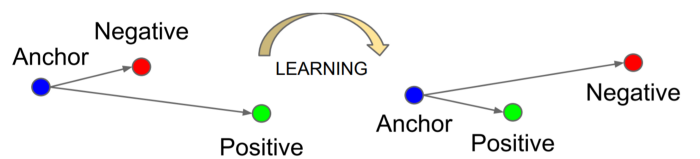
\includegraphics[width=\textwidth]{img/triplet_loss.png}
    \caption[Triplet loss]{The Triplet loss minimizes the distance between an anchor and a positive and maximizes the distance between the anchor and the negative datapoint.\\
    Source: \cite{tripletlossnn}}
    \label{fig:triplet_loss}
\end{figure}

This is the basic idea behind the triplet loss introduced by \cite{tripletlossfirst} and then further formalized by \cite{tripletlosssecond} and subsequently used as a loss function for \glspl{nn} by \cite{tripletlossnn}.

We shall use the triplet loss in following form:
\begin{defn}
Triplet loss for selected triplet (A, P, N) is:
\begin{equation}
\mathcal{L}(A, P, N) = \text{max}(\delta(f(A), f(P)) - \delta(f(A), f(N)) + \alpha, 0)
\label{eq:triplet}
\end{equation}
Where $f$ is a transformation given by \gls{nn}, $\delta$
is a selected distance function and $\alpha$ is a priori selected threshold. The
selected triplet is a triplet of specific samples -- $A$ is a generic point
called ``anchor'' point, $P$ is a ``positive'' sample (i.e. sample of the same
cluster as anchor point) and $N$ is a ``negative'' sample (i.e. sample of
different cluster than anchor point).
\end{defn}


Such a definition provides the formula of the loss for a specific triplet. However, we can easily extend this notion by considering the average loss over all selected triplets.

It can be easily seen that the minimal value of the Triplet Loss is zero. In order to achieve this optimal value, not only do all ``in-between'' clusters distances have to be greater than ``within'' cluster distances, but they must be greater by at least a given margin $\alpha$.

\subsection{Triplet Selection}

An additional challenge for using Triplet Loss is to select suitable triplets. Usually, each point in the dataset (or more precisely in a subset of the dataset called a batch) is once selected as an anchor point. Then the task is then to find the appropriate positive and negative sample for each anchor point.

The related terminology is somewhat ambiguous. For practical purposes, we chose to use the terminology corresponding to the implementation in the Tensorflow framework (\cite{tensorflow}). They operate with two strategies: Hard and Semi-Hard Triplet Loss.

In the case of Hard Loss, the positive and negative samples are selected ``as hard as possible'', which means that the positive sample is the furthest (from the anchor point) out of all considered samples of the same cluster. On the other hand, the negative sample is the closest sample out of all samples from samples that are not of the same cluster as the anchor point.

The Semi-Hard approach selects such a pair of positive and negative samples that the negative sample is further away from the anchor point than the positive one, but not by the required margin. In terms of \autoref{eq:triplet} it means that $\delta(f(A), f(P)) < \delta(f(A), f(N))$ and $\delta(f(A), f(N)) - \delta(f(A), f(P)) < \alpha$.
\chapter{Related Work}

\label{ch:related_work}

%123456789 123456789 123456789 123456789 123456789 123456789 123456789 123456789

Great advantages offered by the usable re-identification algorithm also bring a considerable amount of research in the area. In this chapter, we aim to review this research and related articles. Furthermore, we also focus on the popular architectures of \glspl{nn} for image processing (not necessarily targetted for \reid{}).


\section{Person \Reid{}}

\label{sec:person_reid}

The problem of \reid{} has been an active research area for the past few decades and still is today. Many different approaches were explored by this date. Most of the designs embed the input image of the person into a specific feature space. Resulting feature vectors are then compared using some standard distance function. In combination with a suitably selected threshold, this produces the desired answer whether there is the same person on selected images or not (\cite{cheng2016person}). However, even designs that seek to directly answer the question without embedding the images into some intermediate feature space were explored (\cite{li2014deepreid}).

\subsection{Early Research}
\label{sec:early_research}

Many early attempts in tracking and re-identification describe the images using colors and color histograms in particular. For example, work presented by \cite{krumm2000multi} shows the usage of color histograms to perform tracking in the indoor environment.

Another interesting research was shown by \cite{orwell1999multi}. Again the authors extract color histograms. These histograms are then matched to identities by using \gls{em} over a set of Gaussians.

Even though the use of color histograms was later somewhat overshadowed by more complex techniques such as deep learning, some researchers still use it to perform \reid{}. For example, \cite{zeng2014person} combines the color histogram with spatial information to obtain better results.

Aside from the color histograms, we can see a variety of new techniques emerging. A technique based on the principal axes is presented by \cite{hu2006principal}. Ability to correctly identify the axes heavily relies on successful filtering out the background. The filtering is especially challenging in the scenarios where the occlusion is present or if people move in crowds. The authors propose a special version of the approach to tackle these challenging scenarios. Once the silhouette of a person is established, the principal axis is found. The algorithm then infers the position of the ``ground-point'', i.e., the point where the person touches the ground (this is usually the point where the principal axis intersects the lower bound of the bounding box but it may not be so simple in the case of occlusion). Based on these ``ground-points`` with the use of the Kalman filter, the algorithm then tracks the people. In order to re-identify the person across multiple cameras, the homography is firstly computed using suitable landmarks. Based on this obtained homography, it is straight-forward to compute the sets of points in each camera's view corresponding to the same ``ground-point''. A simple algorithm for maximum likelihood is used to establish a suitable matching (\reid{}) of detected people.

\subsection{Era of the Deep Neural Networks}

More and more successful models based on the deep learning emerged in the past few years. As well as many other image processing task, this field also came to a new era of proposed approches based on \glspl{nn}.

One such research is presented by \cite{ding2015deep}. The authors propose a relatively simple \gls{nn} consisting only of a few convolutional layers, interwoven with the max-pooling layers. To train the network, they use a Triplet Loss (albeit using non-standard terminology). They elaborate more on the selection of the triplets to train on.

A similar approach was explored by \cite{cheng2016person}. The basis of their method is again convolutional \gls{nn} trained by Triplet Loss. However, they presented several notable improvements. Firstly, the architecture they designed after the first convolutional layer ``splits'' the input into four horizontal strips. Meaning that each of these strips is fed into its own independent part of the \gls{nn}, where each part tries to learn the features of its respective body part. However, the original information is also used (``copied'') into the fifth ``global'' part of the \gls{nn} and trained. At the end of the \gls{nn} pipe-line, the parts' outputs are combined. The loss function used is again the Triplet Loss. The authors also focused on the formulation of Triplet Loss. They propose a slightly different formulation of the Triplet Loss, designed specifically for the \reid{} task.

Another \gls{nn} design is presented by \cite{li2014deepreid}. Unlike other approaches, they do not use Triplet Loss or a similar loss to embed the original images into feature space. The architecture they propose directly processes pair of images. The output of the whole network is then simply a number which describes ``confidence'' of the \gls{nn} how likely the images display the same person. Such architecture is then trained via simple softmax loss.

Additional work that tries to solve this problem with the usage of deep \gls{nn} is presented by \cite{hermans2017defense}. They experiment with the hand-crafted architecture of the neural network, as well as the pre-trained ResNet model, (we review ResNet in \autoref{ssec:resnet}). They further elaborate on the topic of Triplet Loss and suitable triplet selection.

Quite elaborate deep network architecture is offered by \cite{xu2018attention}. Their Attention-Aware Compositional Network can be broken into several parts. Firstly, the network tries to estimate an attention map and a visibility score for each body part (given body parts are setup by researchers prior learning). Based on the visibility, the features are extracted for the given parts. Finally, the feature vector representing the original image is produced by selected base network.

\section{Image Processing Architectures}

\label{sec:existing_architectures}

In this section, we further review a few very popular \gls{nn} architectures for image processing. Even though they are not specifically designed for re-identification, we utilize both their architectures and the weights trained for classification tasks that we use via means of the transfer learning (see \autoref{ssec:transfer_learning}).

We present more in detail two well-known \gls{nn} -- MobileNet and ResNet. Both of them presented a break-through in their own category at the time they were introduced.

\subsection{Residual Networks}
\label{ssec:resnet}


Residual networks (commonly referred to as just ResNets) are a quite popular family of \gls{nn} architectures designed especially for processing images. The first ResNet was officially introduced and described by \cite{resnet} and later improved by \cite{resnetimp}. With this model the authors won a few image processing competitions and as such the architecture immediately became very popular. The model won the first places at ILSVRC competition on the tasks of ImageNet detection, ImageNet localization (\cite{imagenetresults}) as well as COCO detection and COCO segmentation at COCO competition (\cite{cocodataset}). To this date this architecture remains inspiration for various state-of-the-art models and approaches.

Next, we investigate the proposed ResNet architecture and the motivations behind it. The authors tried to solve the problem of low training accuracy of the deep neural networks compared to their shallower counterparts. This counter-intuitive phenomenon led them to the following design change.

For a given layer, instead of learning direct suitable mapping $H(\vec{x})$, they designed the layer to learn just the ``residuum'' $H(\vec{x}) - \vec{x} = F(\vec{x})$ (hence the name). This was achieved by adding a residual connection between layer $n$ and layer $m > n$. The output of layer $n$ and layer $m - 1$ would be added together (see \autoref{fig:resnet_schema}), effectively pushing the layer $m$ to learn the residuum with respect to the output of layer $n$ rather than the whole original function.

\begin{figure}
    \centering
    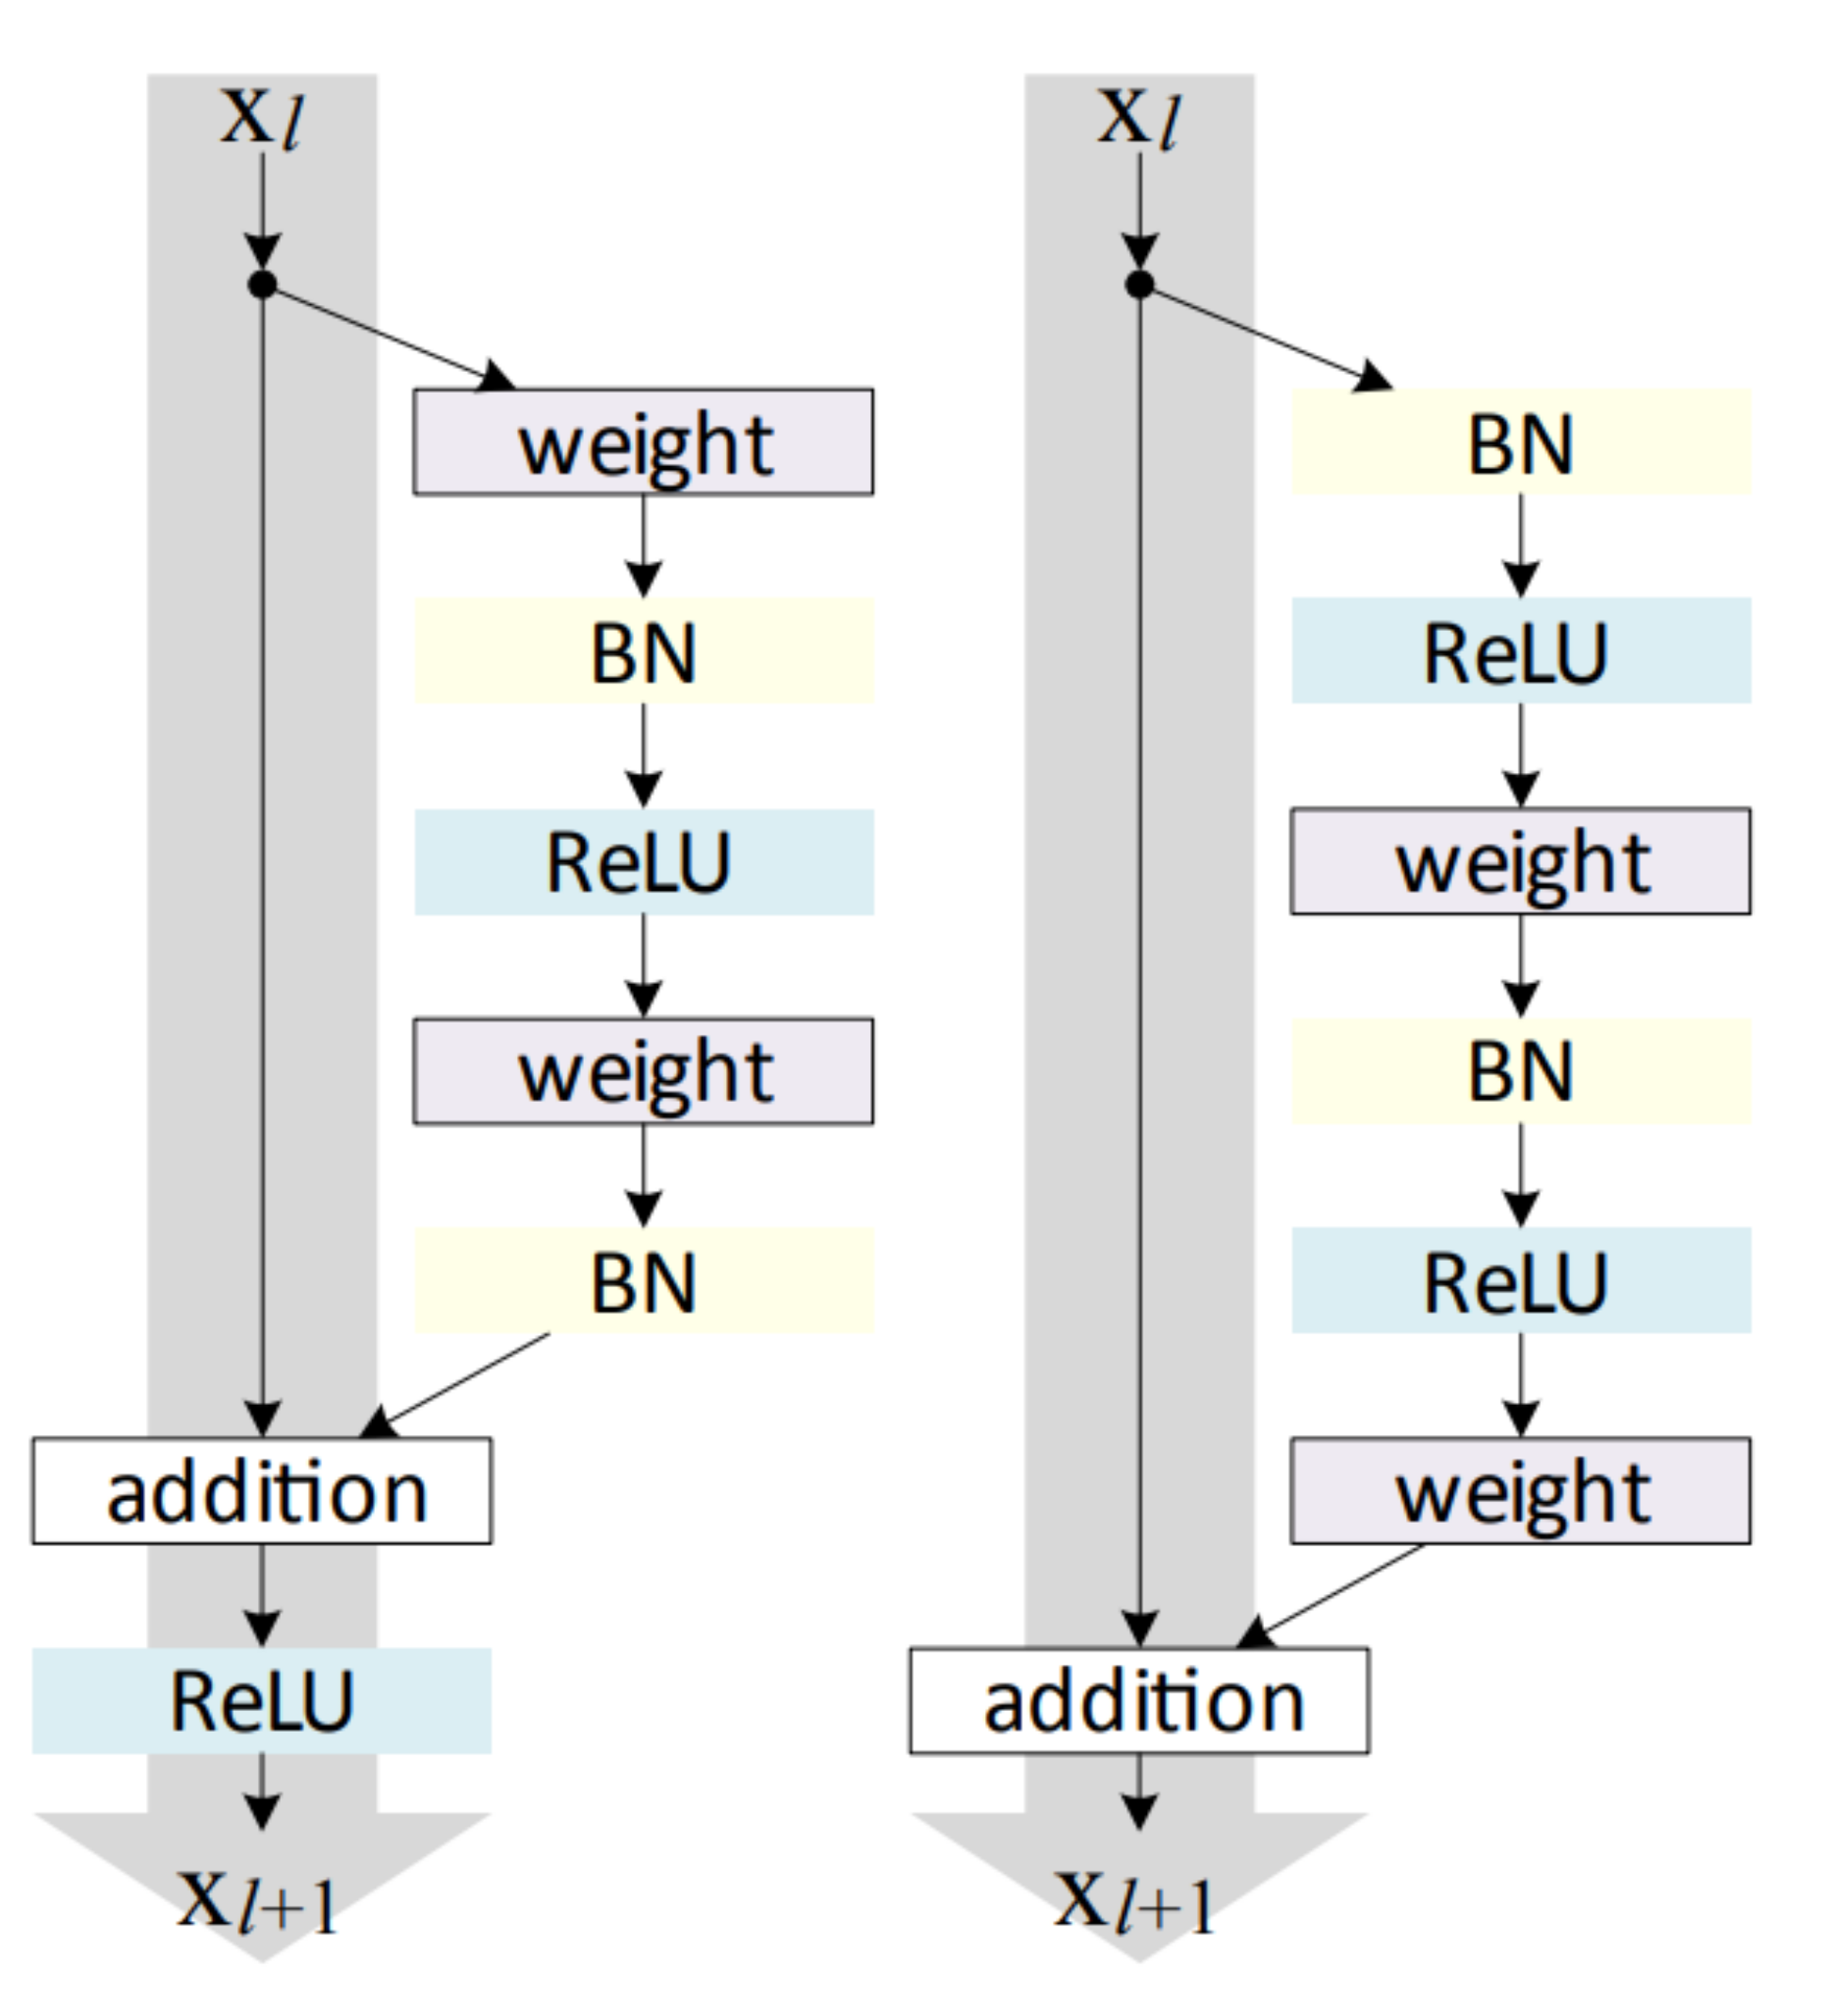
\includegraphics[width=0.48\textwidth]{img/resnetv2.png}
    \caption[Residual units]{Schema of the ``residual units''. On the left as presented by \cite{resnet}. The improved version by \cite{resnetimp} is on the right. Source: \cite{resnetimp}}
    \label{fig:resnet_schema}
\end{figure}

The rationale behind this change is that by adding layers that perform identity function, we can not worsen (or change at all for that matter) the network's output. Therefore, if we take a shallow network and increase its complexity by adding new layers, the (training) error should not decrease if the learning to approximate identity function is easily achieved. However, as the training error increases in traditional design, it can be argued that learning identity function is quite hard using gradient descent algorithm. By adding the residual connection, the problem of learning to approximate identity function becomes just a task of driving the weights of the connections to zero, which should be easier than to learn the identity function directly. As already mentioned, this rationale was successfully empirically proved on several tasks.

The original authors further improved this design in \cite{resnetimp} by reorganizing the layers in the network. They removed the activation function from the residual connection (or, more precisely, they moved it to the ``skipped'' part of the \gls{nn}). This way, they simplified the shortcut even more (see \autoref{fig:resnet_schema}). They further support this change by thorough empirical testing. Since then the ResNets and their derivates became an iconic break-though in deep learning.

\subsection{MobileNets}

\label{ssec:mobilenet}

Other notable architectures are MobileNets by \cite{mobilenets}. In these architectures, authors successfully created models with relatively low latency while maintaining a high accuracy level. The motivation behind such architecture is to provide suitable models for usage in mobile vision applications. They achieved the lowered latency of inference by simplifying some operations in the \gls{nn}.

The most notable change is the replacement of the standard convolutional layers as described in \autoref{sec:conv} by a pair of layers -- depthwise convolutional filter and pointwise convolutional filter.

In the first of these layers -- depthwise convolutional filter -- the convolution is applied on each input channel separately:

$$y_{i, j, r} = \sum_{k, l} x_{i+k, j+l, r} \, c_{k, l, r}$$
The latter of these two layers -- pointwise convolution filter -- is just simple convolution with kernel of size $1 \times 1$.

This replacement of the convolutional layer by two simpler layers significantly decreases the computation cost of inference and the time required for training such a network. The high accuracy of the resulting \glspl{nn} was empirically verified on the ImageNet tasks.

This architecture was then further improved by \cite{mobilenetv2} by introducing inverted residuals and linear bottlenecks. As these concepts are quite complex, we refer the reader to the original article for more information.


\section{Object Detection}

In this thesis, we focus on actual \reid{} within the stream. Prior to the \reid{} the object must be located within the stream itself. For this purpose, we use a third-party neural network. In particular, we use the network designed by \cite{dobransky2019}. The network is based on the Single Shot Detector (\cite{liu2016ssd}) adjusted to the ResNet architecture for low latency to allow real-time video stream processing. As object detection is not a topic of our work, we shall refer the reader to the original work for more details.


\chapter{Formulation and Workflow}

%123456789 123456789 123456789 123456789 123456789 123456789 123456789 123456789
Here we present a formal description of our task and the basic overview of the proposed framework. In this context, we also briefly review the \gls{VL} system as our work is intended to work as its module.

\section{Videolytics}

\label{sec:vl}

Our work is designed to fit into \gls{VL} \todo{by ??} -- an analytical system for video processing and advanced analytics. The goal of the system is to offer an effective way to produce an answer for various queries. Such requests may range from showing an advanced user interface for a live stream to retrieving statistical data from videos stored for offline processing. In order to compute all needed information, the system utilizes various \gls{ml} models. The system may be used to enhance the basic capabilities of security cameras and provide better data that can be utilized in various areas of city planning.

\Gls{VL} is designed as a modular system. This modularity is achieved by using a database as a core component of the system. Modules use the database as the only means of exchanging information. Such a solution makes it easier to add new modules, as their implementations are independent (aside from the \gls{api} defined by the database tables). An additional advantage of this approach is that it makes the data persistent and, therefore, it possible to re-evaluate any experiments.

\section{Task formulation}

Our goal is to implement the re-identification module for the \gls{VL}. As described in the Introduction, re-identification is, in essence, matching the same object across different frames. To focus directly on the re-identification, we use the stream pre-processing offered by the \gls{VL} system.

\subsection{Input}

\label{ssec:input}

%123456789 123456789 123456789 123456789 123456789 123456789 123456789 123456789
Firstly, let us describe the input of our module. To focus directly on the re-identification task, we use other modules to detect an object within the streams and crop out the relevant part of the frame. The input for our part of the system is then just the cropped images alongside additional metadata. We shall refer to this pre-processed input throughout the thesis as \glspl{det}. Let us formally define this notion of \glspl{det}.

Arguably the most important part of the \gls{det} is the image (crop) of the detected object. As \gls{VL} offeres the system for selecting axis-aligned minimal bounding boxes of interesting objects, we focus on rectangular images only. We shall define universe of rectangular images $\mathcal{I}$, using standard RGB representation:

\begin{equation}
\mathcal{I} = \bigcup_{\substack{n \in \mathbb{N} \\ m \in \mathbb{N}}} \{0, 1, \ldots, 2^8-1\}^{3mn}
\label{eq:image}
\end{equation}


This representation describes an image as a matrix of pixels where each pixel is further split into triplets, each element describing one channel (red, green, and blue).

We formalize the notion of the source of the original stream (i.e., camera or the video file) where the detection comes from. For the given task, the only relevant information is the dimension of the stream. Aside from that, we assign each camera a unique identification number (to reflect the fact that we can indeed work with two different cameras of the same dimension). We can then formally define the universe of sources as:

$$\mathcal{C} = \{c_i, c_h, c_w \mid c_i \in \mathbb{N}, c_h \in \mathbb{N}, c_w \in \mathbb{N}\}
 = \mathbb{N}^3$$
 
We shall also refer to sources as cameras interchangeably due to consistency with the other work in the area and the underlying implementation.

%123456789 123456789 123456789 123456789 123456789 123456789 123456789 123456789
The final component of the \gls{det} is the additional metadata. For each detection, we record the relative position $x_0, y_0$, of the top left corner of the detection within the stream. Similarly, we denote $x_1, y_1$ relative position of the bottom right corner. Furthermore, we store a \emph{class} by each detection-- representing the detected object's class. Such class is an element of pre-defined vocabulary $V$. Our vocabulary is defined by pre-processing modules of the \gls{VL} systems. It is a relevant subset of classes used in the COCO dataset by \cite{cocodataset}:

$$V = \{\text{``person'', ``motorcycle'', ``car'', ``truck'', ``train'', ``bicycle'', ``bus''\}}$$


The last component of the metadata is a timestamp $t \in \mathbb{R}^+$. Note that technically we store the timestamp to a certain degree of precision. Therefore, we can consider $t \in \mathbb{N}$. This notation allows us to define the universe of metadata~$\mathcal{M}$ as:

$$\mathcal{M} = \{{(x_0, x_1, y_0, y_1) \in [0,1]^4 \mid x_0 < x_1 \land y_0 < y_1}\} \times V \times \N \times \R$$

The first quadruplet represents the position, then a class mentioned, followed by the camera's identifier, and the last number represents the timestamp.

Now, we can define the universe of \glspl{det} $\mathcal{D}$ as combination of images and metadata:

$$\mathcal{D} = \mathcal{I \times M}$$

\subsection{Task}

\label{ssec:task}

As usual in \gls{ml} tasks, we formulate our goal via a pair of input and the desired output (so-called ``golden truth''). Here we present an important distinction of our algorithm to the standard re-identification approach presented in the Introduction and \autoref{sec:person_reid}. The result of standard re-identification is a learned function that predicts if two input \glspl{det} are of the same object or not. On the other hand, our approach takes into consideration all presented \glspl{det} at the same time and partitions them based on the displayed object. It essentially works as a form of clustering.

Usually, the set presented on the input of our algorithm is a set of \glspl{det} extracted from simultaneous recordings from the cameras placed close together (i.e., we can expect objects to move from one camera to another or even to be recorded by multiple cameras at the same time). Working in the context of the whole set of \glspl{det} gives our algorithm an extra piece of information during the inference. For example if two \glspl{det} $d_0, d_1$ are visually different but both are similar to a third \gls{det} $d_2$, we may then conclude that $d_0$ and $d_1$ display the same object (as well as $d_2$) which we may not find out if we did not consider $d_2$.


As mentioned, to actually formalize our goal, we consider ``golden'' partition~$A$ of given \glspl{det}~$D$. This partition represents true re-identification of input \glspl{det}, i.e. an element~$a \in A$ contains all \glspl{det} that display one object. Our algorithm's goal is then to find this golden partition based on the input \glspl{det} $D$. Throughout the thesis we shall refer to any partition of set of \glspl{det} (both, the ``golden'' partition and the imperfect approximation our algorithm generates) as \glspl{iden}.



To summarize this concept, we shall refer to a pair of set of related \glspl{det} and the associated golden partition $A$ as a \gls{ses}. Formally we can define the universe of all theoretically possible \glspl{ses} $\mathcal{S}$ as:

\begin{equation*}
\begin{split}
&\mathcal{S} =\\& \left\{D \subset \mathcal{D},\,A \subset \mathcal{P(D)} \mid (\forall a \in A) (\forall a' \in A) (a \neq \emptyset) \land (a \cap a' = \emptyset) \land \left(\bigcup A = D\right)\right\}    
\end{split}
\end{equation*}


Our algorithm then works in context of one \gls{ses}~$S = (D, A), S \in \mathcal{S}$. A set of \glspl{det}~$D$ is given to the  algorithm and the goal is to recreate the hidden golden identities~$A$. Our algorithm assigns arbitrary identification number to each identity, therefore we can formalize the desired output as following clustering function~$r_D^*$:

\begin{equation}
\begin{split}
&r_D^*: D \rightarrow \N \text{ s.t. }\\
&(\forall d \in D) (\forall d' \in D) ((r_D^*(d) = r_D^*(d')) \Leftrightarrow (\exists a \in A) (\{d, d'\} \subseteq a))
\label{eq:reidentification}
\end{split}
\end{equation}
Reconstruction of perfect function $r_D^*$ proves to be a hard problem, 
therefore we focus on construction of some approximation $r_D$. We shall further discuss how to measure quality of such approximation in
\autoref{ch:evaluation}. \todo{check this after evalutaion}

As we previously noted this definition of re-identification task differs from the standard definition where we are given just two \glspl{det} and should output if given \glspl{det} are of the same object or not. However we can easily obtain the standard formulation once we obtain our output function $r_D$ as follows:

$$
r_D' : D^2 \to \{0, 1\} \text{ s.t. } (\forall d \in D) (\forall d' \in D) ((r_D'(d, d') = 1) \Leftrightarrow (r_D(d) = r_D(d')))
$$

So far, we have presented our task's definition in the context of already given \gls{ses}. This definition as-is is enough for the work presented in this thesis as we work only with a few selected \glspl{ses}. Nevertheless, we proceed to shortly define the general case in this setting to provide building blocks for future work and motivation for some of our decisions. In a general case, we should not focus on one specific \gls{ses}, but we aim to design an algorithm that works across \glspl{ses}.


However, there is no algorithm that would output suitable $r_D^*$ as in \autoref{eq:reidentification} for all the \glspl{ses}. To see that we just take any distinct pair of \glspl{det}~$D^\bot = \{d_1, d_2\}$. There exists two distinct partitioning and corresponding \glspl{ses}: $S_1 = (D^\bot, \{\{d_1, d_2\}\})$ and $S_2 = (D^\bot, \{\{d_1\}, \{d_2\}\})$. The output function $r_D$ of any algorithm can satisfy \autoref{eq:reidentification} either for $S_1$ or $S_2$ not for both.


Therefore, we shall consider only ``possible'' \glspl{ses}. To properly define such \glspl{ses}, we shall assume some distribution $p_\mathcal{S}$ of \glspl{ses} (this distribution should reflect the distribution we aim the algorithm to work on, i.e. distribution of the \glspl{ses} in the real world). We can define possible \glspl{ses}~$\mathcal{S'}$ as:

$$\mathcal{S}' = \{S \in \mathcal{S} \mid p_\mathcal{S}(S) > 0\}$$
If every set of \glspl{det} is in at most one \glspl{ses}, i.e.:

\begin{equation}
    (\forall (D, A) \in \mathcal{S}')(\forall (D', A') \in \mathcal{S}') (D = D' \Rightarrow A = A'),
    \label{eq:uniq_session}
\end{equation}
Then we can formulate our task by requiring the output function to hold
condition in \autoref{eq:reidentification} for all
\glspl{ses} from $\mathcal{S}'$.

For an (arguably odd) case that \autoref{eq:uniq_session} does not hold, we
define most likely partition for any set of \glspl{det}, given the distribution
of \glspl{ses}~$p_\mathcal{S}$: 

\begin{equation}
A^*_D = \text{argmax}_A \pr_{(D', A')\sim p_\mathcal{S}} \left[A' = A \mid D' = D\right]
\label{eq:mla}
\end{equation}

We can then obtain the valid task definition. We just replace the
\glspl{iden}~$A$ in \autoref{eq:reidentification} by the most likely
\glspl{iden}~$A_D^*$ and require the condition to hold over all sets of
\glspl{det} from possible \glspl{ses}:

\begin{equation}
(\forall d \in D) (\forall d' \in D) ((r_D^*(d) = r_D^*(d')) \Leftrightarrow (\exists a \in A_D^*) (\{d, d'\} \subseteq a))
\label{eq:formulation-final}
\end{equation}


Such definition is in agreement with the definition presented for the case where condition in \autoref{eq:uniq_session} holds.


Finally, let us note that as we picked recordings (and corresponding \gls{ses}) for evaluation of our algorithm randomly, the results of such evaluation reflect the quality of the algorithm with respect to the task as defined by \autoref{eq:formulation-final}.


\section{Workflow}

\label{sec:workflow}

%123456789 123456789 123456789 123456789 123456789 123456789 123456789 123456789

In this section, we describe the general workflow of our re-identification algorithm. Note that, in this thesis, we present several different approaches for the task at hand. This section serves as an overview of the common workflow. Each step is then discussed more in-depth further in the thesis. For the diagram of the worflow, refer to \autoref{fig:workflow}.

\begin{figure}
    \centering
    \def\svgwidth{\textwidth}
    \input{workflow.pdf_tex}
    \caption[General workflow of our re-identification algorithm]{General workflow of our re-identification algorithm. Solid lines represent primary, intended dependencies.
    Dashed lines mark secondary, optimal dependencies, that some algorithms may use.}
    \label{fig:workflow}
    \todo[inline=true]{Remove the word ``Spatial'' from the image}
\end{figure}

Firstly, we shall extract the feature vectors from the images of the \glspl{det}. Such a feature vector should sufficiently describe the image as we shall not use the images directly further in the pipeline. There are several advantages of such representation. They primarily stem from the fact that once the feature vectors are extracted, the original images can be discarded. For one thing, we can lower the memory consumption for storing the data if the extracted feature vectors are smaller than the original cropped images. Another advantage is --- assuming that the feature extraction is an irreversible operation --- that it produces a layer of anonymization, which may be crucial for our task as we work with potentially sensitive data.

After this feature vector extraction, we proceed to actual re-identification. We usually split this process into two parts (we shall describe each step further in the thesis).

The first part is to group \glspl{det} that are close together (i.e., they originate from the same camera, have a very similar position within the frame, and have similar timestamp). We refer to this preliminary grouping as \emph{trajectories}. Although some very advanced strategies can be used even for this stage of the grouping, we shall only work with straight-forward approaches and focus more on the second step. We leave the experimenting with more thought-through approaches (e.g., other algorithms offered by \gls{VL}) as feature work.


The final step is then to group generated \emph{trajectories} into \emph{identities}. As in this step, we need to be able to merge trajectories of the same object across multiple cameras, making the spatial metadata of the \glspl{det} less useful --- we shall focus more on the information of the actual images of the \glspl{det}.

While this split is a bit arbitrary, it arises from practical use. We can use a straight-forward yet precise algorithm while we do not rely on the visual information for the first step. In the second step, we can leverage the fact that we have significantly fewer (by a few magnitudes) objects to merge.

\chapter{Feature Extraction}

%123456789 123456789 123456789 123456789 123456789 123456789 123456789 123456789

\label{ch:features}

In this chapter, we focus on the first step of the workflow described in the \autoref{sec:workflow}. The goal of this step is to represent useful information from an image of a tracked object in the form of a single feature vector. We aim to extract such feature vectors that would be close together (in terms of a suitable distance) if and only if they display the same person.

In this thesis, we use the feature vectors exclusively from the space of real numbers. Therefore, the form of the feature extraction function can be written as:

$$f : \mathcal{I} \goto \R^n \, \text{ for some } n \in \N$$

Where $\mathcal{I}$ is the space of images as in \autoref{eq:image}

\section{Histograms}

\label{sec:histograms}

The first set of feature extraction approaches focuses on encapsulating the distribution of color within a given image. The idea is that the color distribution of the tracked person's image should not change even if the given person moves within the display. We describe this distribution in the forms of histograms, similarly to other research (see \autoref{sec:early_research}).

\begin{figure}
    \centering
    \def\svgwidth{\columnwidth}
    \scalebox{0.6}{\input{img/histogram.pdf_tex}}
    \caption[Visualization of histogram of data]{Visualization of histogram of data $(2, 3, 11, 15, 17, 23)$ with 3 bins, lower bound 0 and upper bound 30. The values of the histogram are $(2, 3, 1)$}
    \label{fig:histogram}
    \todo[inline=true]{Uhladit obrazek}
\end{figure}

Histograms are often used for visualization purposes. However, in this work, we use histograms as actual feature vectors. To avoid any ambiguity, we offer the following definition, which is in line with the standard concept of histograms. An example of histogram accompanied by standard visualization can be seen in \autoref{fig:histogram}.

\begin{defn}
\label{defn:simplehistogram}
Simple histogram of (multi)set $X \subset \R$ of n bins with lower bound $l$ and upper bound
$u$ is a vector $\vec{h}$ with following elements:
$$h_i = \abs{\left\{x \in X \mid l + (i-1) \cdot \frac{u-l}{n} \leq x < l + i \cdot \frac{u-l}{n}\right\}}$$
\end{defn}

However, defining histogram just over the multi-set of real numbers proves to be too restrictive for our needs. For example, in our standard representation of images, each pixel consists of three real numbers (color channels). Our original definition allows only to draw histograms out of a set of real numbers (rather than triplets of real numbers).

One way to circumvent this problem is to draw a histogram from each channel separately and concatenate them together. However, this naïve approach losses valuable information. For example, an image with half red and half green would generate the same histogram as an image that is half yellow (i.e., the combination of red and green) and half black (if we are using RGB channels).

Therefore, we shall use a bit more complex approach. An approach that would encapsulate the combined color information of each pixel. For this reason we use the following extension of simple histograms:

\begin{defn}
\label{defn:histogram}
Histogram of (multi)set $X \subset \R^m$ of n bins per channel with lower bound
$l$ and upper bound $u$ is a tensor $H$ with following elements:
$$H_{i_1, \ldots, i_m} = \abs{\left\{\vec{x} \in X \mid (\forall j) \left(l + (i_j-1) \cdot \frac{u-l}{n} \leq x_j < l + i_j \cdot \frac{u-l}{n}\right)\right\}}$$
\end{defn}

It is easy to see that the \autoref{defn:histogram} is (for $m = 1$)
consistent with the \autoref{defn:simplehistogram}.

Finally, as we may compare the histograms of images of various resolutions (and thus varying number of pixels), we shall use term of normalized histogram:

\begin{defn}
\label{defn:normhistogram}
Normalized, histogram of (multi)set $X \subset \R^m$ of n bins per channel with
lower bound $l$ and upper bound $u$ is a tensor $\widehat{H}$ with following
elements:
$$\widehat{H}_{i_1, \ldots i_m} = \frac{H_{i_1, \ldots i_m}}{\sum_{j_1, \ldots, j_m} H_{j_1, \ldots, j_m}}$$
Where $H_{i_1, \ldots, i_m}$ is a histogram of $X$.
\end{defn}

\todo[inline=true]{Doplnit srovnani concatenace a multi-d-histogramu do eval.}

\subsection{Color Models}

As we mentioned previously in this section, so far, we aim to capture the distribution of the color within an image via histograms. However, we need to decide how we want to represent the pixels in the first place. We explore several well-known models.

\subsubsection{RGB}

The \autoref{defn:normhistogram} allows us to construct the first feature vector simply by following the definition. We can construct a (three-dimensional) histogram from the original channels (red, green, and blue).

However, such a naïve approach has significant drawbacks. In our scenario, it is common that the tracked object or person changes its brightness. It may move to a shadow or enter the area under a lamp. However, the object does not change its identity by moving to more bright areas. Therefore, we would prefer a model that is invariant to changes in the lightning (or at least not very sensitive). Unfortunately, this is not achieved by considering standard RGB as our color model.


A simple comparison can be seen in \autoref{fig:rubik_rgb_hsv}. In the figure, we work with three photos of the same object in three different light conditions. The original photos are shown in the top row. We can see the decomposition of red, green, and blue channels, respectively, in the following three rows. As we can see, even though we photographed the same object from the same vantage point, the changes in light conditions have a dramatic impact on all three channels.

\begin{figure}
    \newlength{\rubiklength}
    \setlength{\rubiklength}{3cm}
    \centering
    \begin{tabular}{rccc}
         Original &
         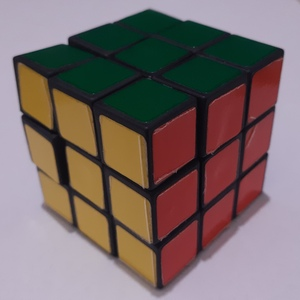
\includegraphics[width=\rubiklength]{img/rubik/1_orig.jpg} & 
         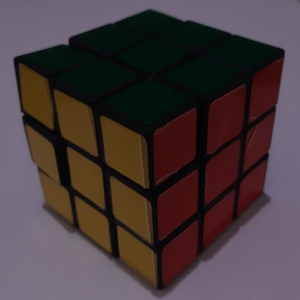
\includegraphics[width=\rubiklength]{img/rubik/2_orig.jpg} & 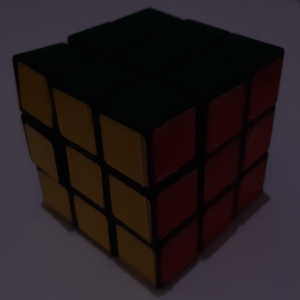
\includegraphics[width=\rubiklength]{img/rubik/3_orig.jpg}\\
         
         Red &
         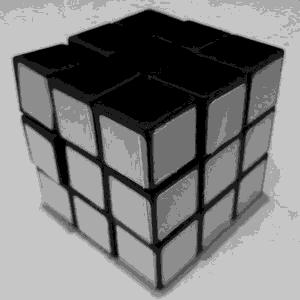
\includegraphics[width=\rubiklength]{img/rubik/1_rgb_r.jpg} & 
         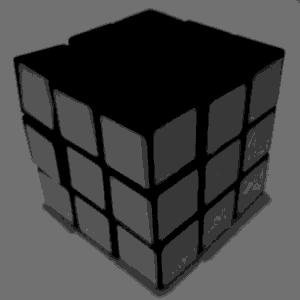
\includegraphics[width=\rubiklength]{img/rubik/2_rgb_r.jpg} & 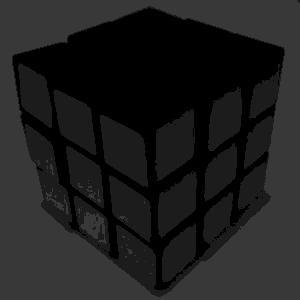
\includegraphics[width=\rubiklength]{img/rubik/3_rgb_r.jpg}\\
         
         Green &
         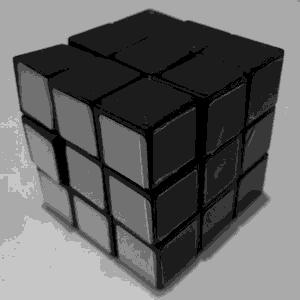
\includegraphics[width=\rubiklength]{img/rubik/1_rgb_g.jpg} & 
         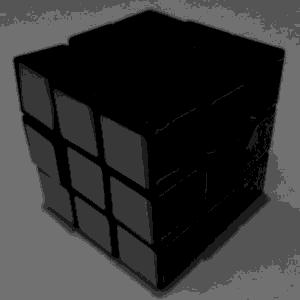
\includegraphics[width=\rubiklength]{img/rubik/2_rgb_g.jpg} & 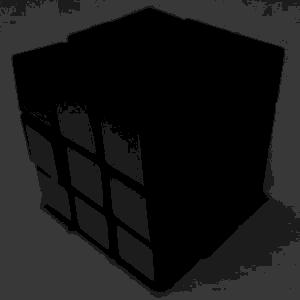
\includegraphics[width=\rubiklength]{img/rubik/3_rgb_g.jpg}\\
         
         Blue &
         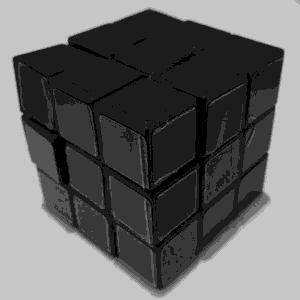
\includegraphics[width=\rubiklength]{img/rubik/1_rgb_b.jpg} & 
         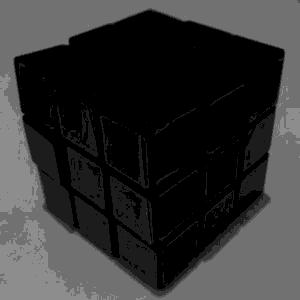
\includegraphics[width=\rubiklength]{img/rubik/2_rgb_b.jpg} & 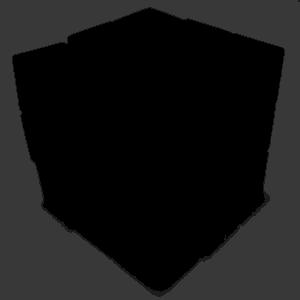
\includegraphics[width=\rubiklength]{img/rubik/3_rgb_b.jpg}\\
         
         Hue &
         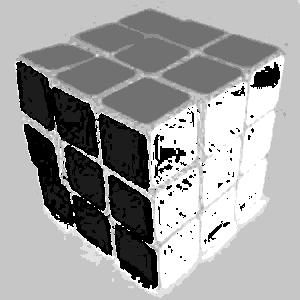
\includegraphics[width=\rubiklength]{img/rubik/1_hsv_h.jpg} & 
         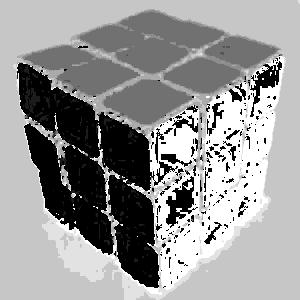
\includegraphics[width=\rubiklength]{img/rubik/2_hsv_h.jpg} & 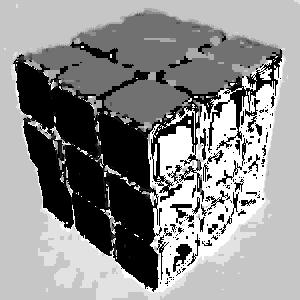
\includegraphics[width=\rubiklength]{img/rubik/3_hsv_h.jpg}\\
         
         Saturation &
         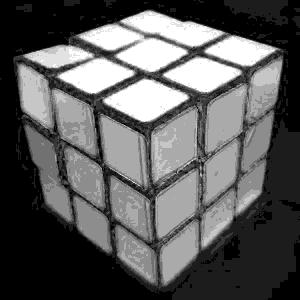
\includegraphics[width=\rubiklength]{img/rubik/1_hsv_s.jpg} & 
         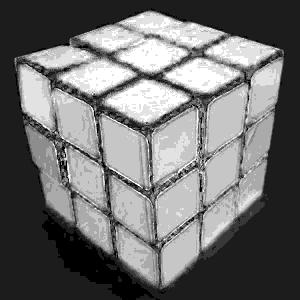
\includegraphics[width=\rubiklength]{img/rubik/2_hsv_s.jpg} & 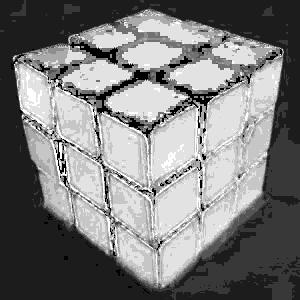
\includegraphics[width=\rubiklength]{img/rubik/3_hsv_s.jpg}\\
         
         Value &
         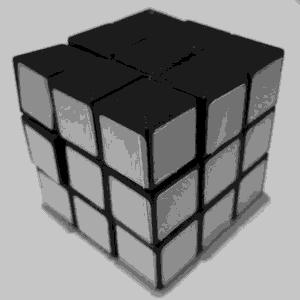
\includegraphics[width=\rubiklength]{img/rubik/1_hsv_v.jpg} & 
         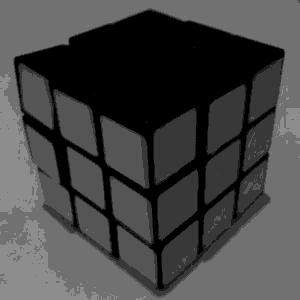
\includegraphics[width=\rubiklength]{img/rubik/2_hsv_v.jpg} & 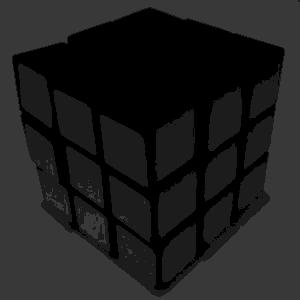
\includegraphics[width=\rubiklength]{img/rubik/3_hsv_v.jpg}

    \end{tabular}
    \caption[RGB and HSV decomposition of an object under varying light conditions]{RGB and HSV decomposition of an object under varying light conditions. The original photos are shown in the top row, the next three
    rows show red, green and blue components (lighter means higher value
    of given component). Last three rows show HSV components.}
    \label{fig:rubik_rgb_hsv}
\end{figure}

\begin{figure}
    \centering
    \setlength{\rubiklength}{3cm}
    \begin{tabular}{rccc}
         Original &
         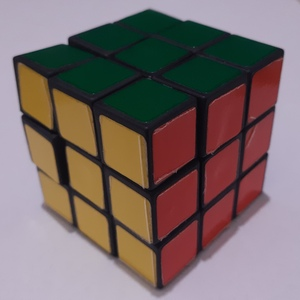
\includegraphics[width=\rubiklength]{img/rubik/1_orig.jpg} & 
         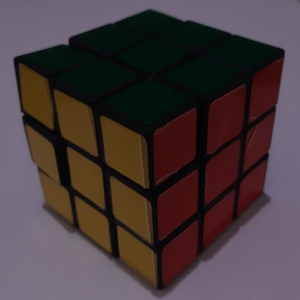
\includegraphics[width=\rubiklength]{img/rubik/2_orig.jpg} & 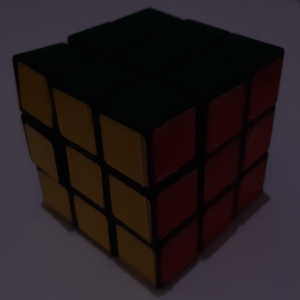
\includegraphics[width=\rubiklength]{img/rubik/3_orig.jpg}\\
         
         Luma &
         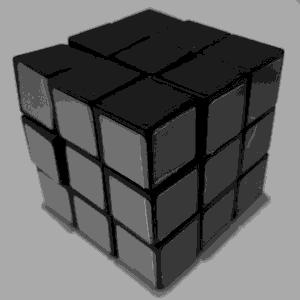
\includegraphics[width=\rubiklength]{img/rubik/1_yuv_y.jpg} & 
         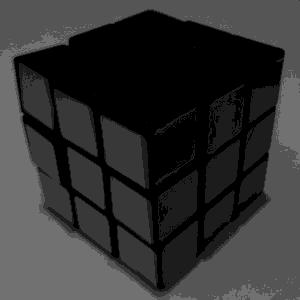
\includegraphics[width=\rubiklength]{img/rubik/2_yuv_y.jpg} &
         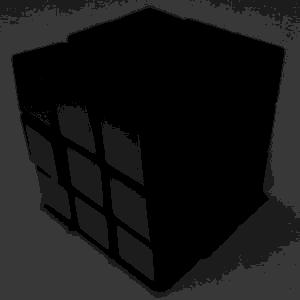
\includegraphics[width=\rubiklength]{img/rubik/3_yuv_y.jpg}\\
         
         Blue projection &
         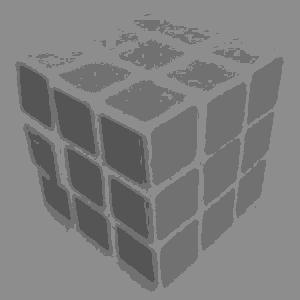
\includegraphics[width=\rubiklength]{img/rubik/1_yuv_u.jpg} & 
         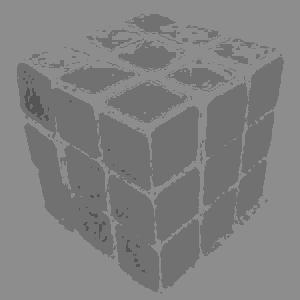
\includegraphics[width=\rubiklength]{img/rubik/2_yuv_u.jpg} &
         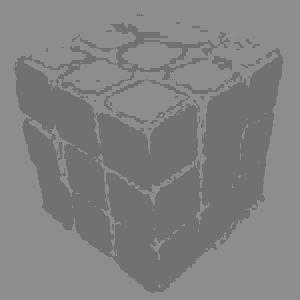
\includegraphics[width=\rubiklength]{img/rubik/3_yuv_u.jpg}\\
         
         Red projection &
         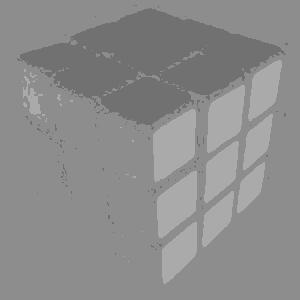
\includegraphics[width=\rubiklength]{img/rubik/1_yuv_v.jpg} & 
         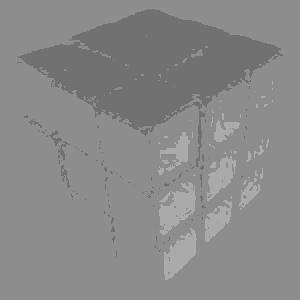
\includegraphics[width=\rubiklength]{img/rubik/2_yuv_v.jpg} & 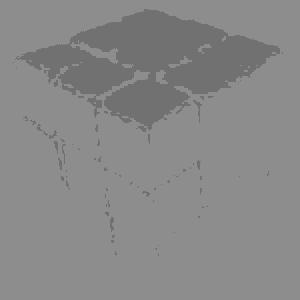
\includegraphics[width=\rubiklength]{img/rubik/3_yuv_v.jpg}
         \end{tabular}
    \caption[YUV decomposition of an object under varying light conditions]{YUV decomposition of an object under varying light conditions. The original photos are shown in the top row, remaining rows show components of luma (Y), blue projection (U) and red projection (V) respectively.}
    \label{fig:rubik_yuv}
    \todo[inline=true]{\LaTeX{} Zarovnat text v prvnim sloupci aby byl vertikalne uprostred (ne dole jak je ted)}
\end{figure}

\subsubsection{HSV}

One of the possible remedies to tackle the problem of changes in the light conditions is to use another popular decomposition of color information -- hue, saturation, and value model. The last value is sometimes referred to as brightness resulting in the abbreviation HSB.\footnote{Another related decomposition is HSL, where the last channel is replaced by lightning. However, as the main channels for our purposes are the first two, we shall not discuss this differentiation any further.} General concept of HSV decomposition is displayed in \autoref{fig:hsv_cylinder}.

The first channel --- hue --- represents what we usually refer to as a main property of the color when we describe it. For example, colors with the hue of $60\degree$ we usually refer to as ``yellow'' and colors with the hue of $120\degree$ we refer to as ``green''.

The hue is often displayed as a direction or a position of the unit circle. Therefore, the unit of hue is most common a degree. This also means that the value of $359\degree$ and $0\degree$ represent nearly identical color (red).

Mathematically we can compute the value of hue from the RGB channels as
follows:

$$H = 60\degree \cdot x, \text{ where } x = 
\begin{cases}
0 & \text{ if } R = G = B \\
\frac{G - B}{R - B} & \text{ if } R \geq G \geq B \\
2 - \frac{R - B}{G - B} & \text{ if } G > R \geq B \\
2 + \frac{B - R}{G - R} & \text{ if } G \geq B > R \\
4 - \frac{G - R}{B - R} & \text{ if } B > G > R \\
4 + \frac{R - G}{B - G} & \text{ if } B > R \geq G \\
6 - \frac{B - G}{R - G} & \text{ if } R \geq B > G
\end{cases}$$

Another component of HSV is saturation. This component describes the ``colorfulness'' of the color. Colors with a low level of saturation always appear to be of grey shade, while the color with higher saturation changes depending on its hue component.

The value of saturation can be easily computed from the RGB components:

$$S = 1 - \frac{\max(R,G,B)}{\min(R,G,B)}$$

We can see that hue and saturation are quite robust in terms of changes in light conditions on the experiment in \autoref{fig:rubik_rgb_hsv}. Furthermore, they describe well the changes in the actual color of the material. That is at least for the simple example of the photo of a Rubik cube. The usefulness of these two channels in practical cases was shown by \cite{mckenna1997tracking}, where the authors used them to re-identify faces.

\begin{figure}
    \centering
    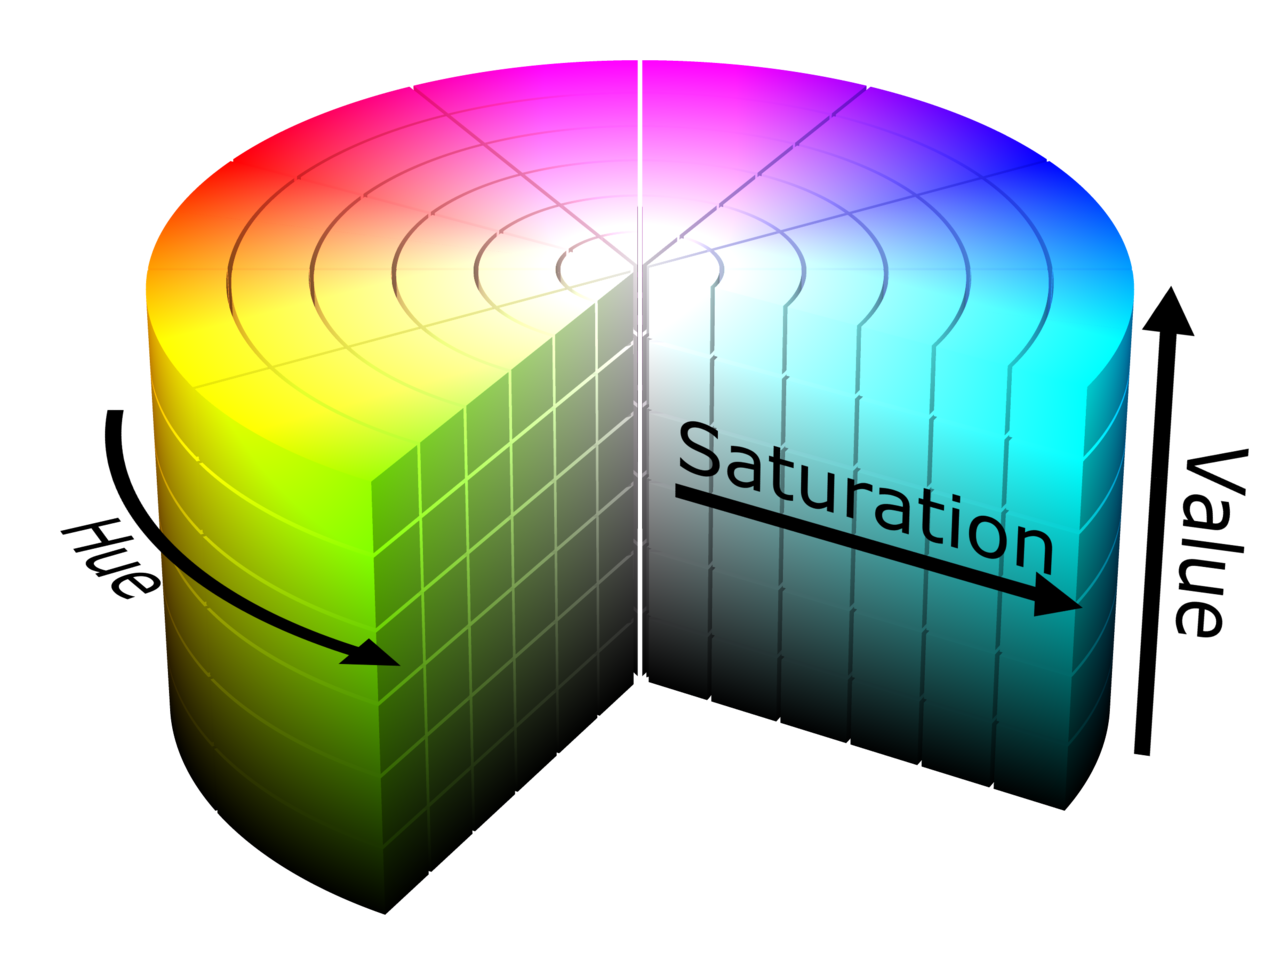
\includegraphics[width=6cm]{img/HSV_color_solid_cylinder.png}
    \caption[HSV color cylinder]{HSV color cylinder\\Source: HSV color solid cylinder\protect\footnotemark{} by SharkD, CC BY-SA 3.0\protect\footnotemark{}, via Wikimedia Commons}
    \label{fig:hsv_cylinder}
    \todo[inline=true,color=cyan]{\LaTeX tenhle zpusob sazeni hodi footnote na jinou stranu nez je obrazek. Lepsi nez to vubec nemit, ale mozna s tim zkusim jeste neco udelat}
\end{figure}
\addtocounter{footnote}{-2}
\stepcounter{footnote}\footnotetext{\url{https://commons.wikimedia.org/wiki/File:HSV_color_solid_cylinder.png}}
\stepcounter{footnote}\footnotetext{\url{https://creativecommons.org/licenses/by-sa/3.0}}

\subsubsection{YUV}

Another fairly popular (\cite{orwell1999multi}, \cite{wren1997pfinder}) encoding of color used for this task is YCbCr (often referred as YUV) system. The first component, Y, represents the luminance (brightness) of the color\footnote{Component Y' is often used in place of the Y component. There is a difference between these two notation; however, we shall not discuss this difference further as the important components for our work is the latter two components.}. The remaining two components represent the chrominance of the color. The first of these two components (U or Cb) represents the blue projection. The last component (V or Cr) represents the red projection. The UV decomposition (with fixed Y) can be seen in \autoref{fig:yuv_decomposition}.

\begin{figure}
    \centering
    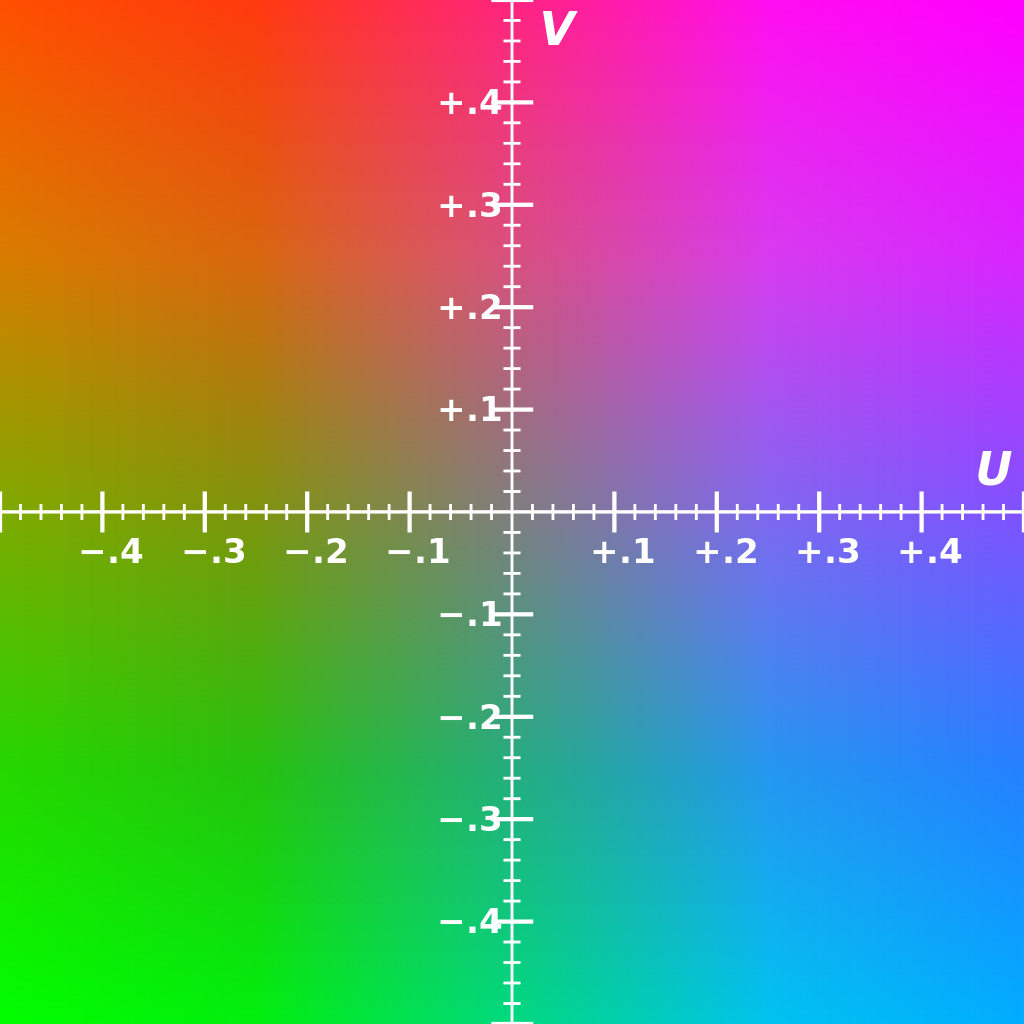
\includegraphics[width=6cm]{img/YUV_UV_plane.svg.png}
    \caption[UV plane of YUV decomposition]{UV plane of YUV decomposition\\
    Source: YUV UV plane\protect\footnotemark{} by Tonyle, CC BY-SA 3.0, via Wikimedia Commons \protect\footnotemark{}}
    \label{fig:yuv_decomposition}
\end{figure}
\addtocounter{footnote}{-2}
\stepcounter{footnote}\footnotetext{\url{https://commons.wikimedia.org/wiki/File:YUV_UV_plane.svg}}
\stepcounter{footnote}\footnotetext{\url{http://creativecommons.org/licenses/by-sa/3.0/}} 

The definition we use in this work comes from ITU-R Recommendation BT.601
(often just Rec. 601; \cite{bt2011studio}). However, we apply linear
transformation with offset and additional rounding to map the original space of U and V
to map these components to 8-bit values. This transformation can be expressed
as:

\begin{align*}
U &= \floor{(-43R - 84G + 127B) / 256} + 128 \\
V &= \floor{(127R - 106G - 21B) / 256} + 128
\end{align*}

How well these channels capture the color information and how much they change with the lightning change can be seen in the \autoref{fig:rubik_yuv}.

\subsection{Background filtering}

There is another aspect to consider when using color histograms for generating feature vectors, and that is background filtering. If we did not filter out the background, the histogram might be polluted with useless information and may change during the tracked individual's movement, thus lowering the re-identification ability of the generated feature vector.

We evaluated the results without any background filtering at all as a baseline. Aside from that, we explore two rather simple approaches to this task. 

\subsubsection{Simple crop}

The first, quite naïve approach is to crop from each image. We can remove strips of fixed width (relative to the image's dimension) from each side. An example of the result of this approach can be seen in \autoref{fig:crop_example}.

This way, we can remove (in most cases) all the background. Unfortunately, we often remove not only the background but also usually at least parts of the tracked individual. However, the basic idea is that the part of the person that remains after the crop should be mostly the same (i.e., displaying the same part) and not influenced by the background at all. Even though we may lose some information by this approach (i.e., if the crop from the bottom of the bounding box is too large, we may entirely crop-out the legs), we aim to verify if the remaining information is enough for re-identification purposes.

\begin{figure}
    \centering
    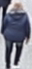
\includegraphics{img/background_filter/1_original.png} $\goto$ 
\includegraphics{img/background_filter/1_small.png} \hspace{2cm} 
\includegraphics{img/background_filter/2_original.png} $\goto$ 
\includegraphics{img/background_filter/2_small.png}
    \caption[An example of cropping on actual detections]{An example of cropping on actual detections. 20\% were cropped from left and right, 10\% from the top and 50\% from the bottom.}
    \todo[inline=true]{\LaTeX{} zarovnat obrazky a sipky vertikalne}
    \label{fig:crop_example}
\end{figure}

\subsection{Weighting by Gaussian}

In the second approach, we assign each pixel a weight. This approach's idea is that the closer the pixel is to the center of the image, the more likely it is that the pixel represents part of the person rather than the background. Therefore, we want to assign higher importance to the pixels near the center.

There are many functions that would generate suitable weights (we need symmetric
function with single local maximum). However, we use one in particular
-- Gaussian (i.e. normal distribution function). We experiment with various
variations of the Gaussian as well as multiple vertical centering points.


To formalize the concept of weighted histograms we further alter the \autoref{defn:histogram}. In the original definition we simply counted the number of pixels corresponding to given bin (i.e. fulfilling the conditions). In the definition of weighted histogram instead of simply counting them, we sum the weights of corresponding histogram. Therefore, if we assign weight 1 to all pixels, resulting histogram would be the same as if we would not use weights at all:

\begin{defn}
\label{defn:weighted_histogram}
Weighted histogram of (multi)set $X \subset (\R^m \times \R)$ (where the last
element of the vector represents weight) of n bins per channel with
lower bound $l$ and upper bound $u$ is a tensor $H$ with following elements:
$$H_{i_1, \ldots, i_m} = \sum_{(\vec{x}, w) \in X} \left[w \text{ if } (\forall j) \left(l + (i_j-1) \cdot \frac{u-l}{n} \leq x_j < l + i_j \cdot \frac{u-l}{n}\right)\right]$$
\end{defn}

A visualization of this weighting can be seen in \autoref{fig:gaussian_weighting}.

\begin{figure}
    \centering
    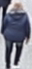
\includegraphics{img/background_filter/1_original.png} \hspace{1cm} 
\includegraphics{img/background_filter/weights.png} \hspace{1cm}
    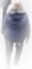
\includegraphics{img/background_filter/weights_applied.png}
    \caption[Visualization of background filtering by Gaussian weighting]{Visualization of background filtering by Gaussian weighting. The chosen distribution is horizontally centered and vertically offset to 30\% of height of the image. Chosen scale of the distribution is 0.3 (with respect to each respective dimensions of the image). The first image shows original image, the second weights, the last one represent applied weights (the weights are represent by transparency channel).}
    \label{fig:gaussian_weighting}
\end{figure}


\section{Neural Networks}



In this section, we explore feature vectors generated by neural networks. The information in these feature vector may not be as easy to understand as in case of using histograms. However, we aim to trade this lower level of explainability in hopes that the resulting feature vector would contain more useful information in terms of \reid{}.


\subsection{Custom architecture}

The first network we evaluate is a simple custom architecture. Our architecture is shallow compared to the more complex counter-parts that we also evaluate. It follows the usual practice of using alternating convolutional, max-pooling, and dropout layers with a dense layer prior to the output. For detailed description of the layers please consult \autoref{sec:conv} and \cite{deeplearningbook}. Detailed architecture is described in \autoref{tab:custom_architecture}.

\begin{table}
    \centering
    \begin{tabular}{l|l|l}
         Layer type & Parameters & Output shape \\ \hline
         \emph{Input} & & $n \times n \times 3$ \\
         Convolutional & filters: 64, kernel size: 2 & $n \times n \times 64$ \\
         Max-pooling & pool size: 2 & $\frac{n}{2} \times \frac{n}{2} \times 64$ \\
         Dropout & rate: 0.3 & $\frac{n}{2} \times \frac{n}{2} \times 64$ \\
         Convolutional & filters: 32, kernel size: 2 & $\frac{n}{2} \times \frac{n}{2} \times 32$ \\
         Max-pooling & pool size: 2 & $\frac{n}{4} \times \frac{n}{4} \times 32$ \\
         Dropout & rate: 0.3 & $\frac{n}{4} \times \frac{n}{4} \times 32$ \\
         Flatten & & 2$n^2$ \\
         Dense & output size: 256, without activation & 256 \\
         Normalization & & 256
    \end{tabular}
    \caption[Architecture of custom neural network]{Architecture of custom neural network. Parameter $n$ represents size of the input (the input is expected to be resized to $n\times n$ pixels, with RGB channels).}
    \label{tab:custom_architecture}
\end{table}

This simple architecture is not as complex as fine-tuned architectures such as ResNet and MobileNet. Therefore, we expect to the resulting feature vectors as quality as the well-researched counter-part. However, it serves as a baseline for this type of approach. Furthermore, its simplicity has other advantages. Training takes significantly less time, which allows for a quick initial overview of the results. It also provides low latency during the inference, which is useful if we extend our usage to on-line \reid{}.

\subsection{Pre-trained architectures}

We experiment with various architectures based on the already trained \glspl{nn} (see \autoref{ssec:transfer_learning} and \autoref{sec:existing_architectures}).

The first experiment in this regard is to use ResNet and MobileNet as they were trained on the ImageNet dataset without the last ``classification'' layer. By such an experiment, we can hypothesize if these networks extract enough information simply by virtue of being image distinguishing neural networks or whether additional training is needed.

Finally, we explore the possibility of improving the abilities of \gls{nn} by fine-tuning them on our dataset. The first straight-forward approach we tested was to train the network without the last ``classification'' layer on our dataset without additional modification.\footnote{Actually in order to employ Triplet Loss for learning, we needed to add a normalization layer. However, this layer does not add any trainable parameters.} However, we also explore the possibilities of slight modifications. We add a custom dense layer, sort of ``in place'' of the removed classification layer.

We also experimente with the so-called ``freezing'' pre-trained part of the model. This means that by learning, we only fine-tuned the added final layer instead of the whole model. This has the advantage of a faster learning as the number of trainable parameters are significantly lower and the derivative has to be computed only for the last layer. Furthermore, using completely untrained weights in the final layer may cause the weights set in the pre-trained part to re-learn and completely lose the pre-trained model's advantages.

\subsection{Training}

We shall train and fine-tune presented models via gradient descent algorithm. To provide an unbiased estimation of the quality of the model in terms of \autoref{eq:mla}, we evaluate entirely different \gls{ses} than we used for training and fine-tuning. Both the training \gls{ses} and the \gls{ses} used for evaluation was created from our recordings. We have manually annotated extracted \glspl{det}. We describe the datasets more in \autoref{sec:datasets}.

For training itself, we use Triplet Loss as described in \autoref{sec:triplet_loss}. We extract the \gls{det} from single (``training'') \gls{ses} for the training purposes. As the goal of this step in the workflow is to obtain the representation of images, we discard all the metadata (e.g. position of the \gls{det}) and leave only the images of the \gls{det}.


Usually, we train the neural networks until the convergence of the loss function is reached. However, in some cases (notably, while incorporating the ResNet architecture), we needed to end the training earlier due to high hardware and time demands. Nevertheless, to avoid overfitting on the training dataset, we also evaluate the networks with weights learned in earlier training stages.

\subsection{Resizing Images}

Many \glspl{nn} for image processing (including those we work with) require the input image to be of fixed dimensions. For resizing images, various algorithms can be employed. We exclusively use the bicubic interpolation to achieve good results when scaling up (which is our common use case). For details please refer to \cite{keys1981cubic}. Other algorithms can be experimented with. However, it is out of the scope of this work.
\chapter{Identity and Trajectory Construction}

\label{ch:iden_construction}

%123456789 123456789 123456789 123456789 123456789 123456789 123456789 123456789

In this chapter we discuss actual techniques to group the \glspl{det} into
desired clusters, i.e. creating \glspl{iden} as per \autoref{ssec:task}.
We show how we combine the visual information of the image
(\autoref{ch:features}) with metadata to provide \glspl{iden}.

\section{Trajectories}

In this section, we focus on grouping the \glspl{det} together without the use of visual information, i.e. purely based on the metadata. In other words we create trajectories as per \autoref{sec:workflow}. By its nature the \glspl{det} within a single trajectory are from consecutive frames and physically close together, displaying one moving object.

The reason for this step is to group the \glspl{det} together in cases
where the visual information -- processing which may be complicated -- is not
needed. The trajectories then serve as a ``building blocks'' for subsequent merging
processes.


% The trajectories serve as a ``building blocks'' for more
% complicated \glspl{iden}. Due to the way they are constructed the trajectories
% are clusters of \glspl{det} that are physically close together. They are usually
% just list of \glspl{det} from the consecutive frames with just a minor changes
% in position of tracked object in-between the frames.

\subsection{Detection Metadata}

Let us briefly recall available metadata for each \gls{det} as introduced in
\autoref{ssec:input}:

\begin{itemize}
    \item $(x_0, x_1, y_0, y_1)$ -- Position of the bounding box of the detection given by $x$-coordinate of the left and the right edge and the $y$-coordinate of top and bottom edge respectively.
    \item Class of the \gls{det}, e.g., person, car or truck
    \item Camera identifier
    \item Timestamp
\end{itemize}

Let us start with a simplification. For now, we consider metadata of just two \glspl{det} at hand, and we explore if we can find out whether the \glspl{det} display the same object (i.e. in this context whether they belong to the same trajectory). We discuss each part of the metadata separately.

For each metadata we use a separate condition or set of conditions. We conclude that the \glspl{det} show the same object if all the conditions are true. In some cases we show the simple conditions are enough (\autoref{ssec:nonspatial_merging}). In other cases, we derive additional values which we compare with selected thresholds. We find suitable thresholds by experimenting with various settings (we discuss this topic further in \autoref{ssec:spatial_merging}).

Note that, even if some of the conditions for a given pair of \glspl{det} are not fulfilled, we can assign the \glspl{det} to the same trajectory later using transitivity. We elaborate further on this topic in \autoref{ssec:trajectory_generation}.

\subsection{Direct Conditions on Metadata}

\label{ssec:nonspatial_merging}

Let us start with the class of the \gls{det}. The class
gives us the most straight-forward conclusion.
If the two \glspl{det} at hand are of different classes we know for sure
that they can not display the same
object.\footnote{There is a quite
odd case where this seemingly obvious conclusion can be argued against. That
is, for example, when a person enters a car. Based on the actual definition of
the \gls{iden} we may consider it as the same displayed object. As these cases
raise multiple questions (e.g. what should happen when multiple people enter the same vehicle), we shall consider a person entering the vehicle and the vehicle itself as different
\glspl{iden} and we leave further research in this topic for a
future work.} As a corollary, we therefore assume that the two \glspl{det} are
of the same class while investigating the rest of the metadata.

We can incorporate camera identifier just as easily. If the two
\glspl{det} are from different cameras, we do not explore the remaining
metadata, as they do not hold any useful information in such
case.\footnote{There
are approaches that assume that the two given cameras capture largely the same
area and are calibrated (for example \cite{hu2006principal}). However, we
assume no prior calibration and therefore we leave similar approaches for other
work.} For example even if there is one detection in top left corner of one
camera, and in the exact same time there is another detection in top left corner
of a different camera, we can not say if the \glspl{det}
display the same person or not. This is
because we do not know if the area within top left corner corresponds to the
area in the top left corner of the second camera. In such case we have to use
a priori assumption and assign them to two different
trajectories.\footnote{Unless we have any additional information the a priori
assumption that two \glspl{det} belong to different golden \glspl{iden} (and thus also a trajectory) is more
likely to be true than the opposite. This holds at least under the assumption that there is no
golden \gls{iden} that would represents more than half of the
\glspl{det} within given \gls{ses}.}

For an assignment into the same trajectory we therefore consider only \glspl{det}
from the same camera. We only elaborate on such cases in the remainder
of this subsection. We discuss the cases how to discover the same object across
different cameras later in this chapter (\autoref{sec:generating_identities}).

Lastly, let us consider additional information that we gain by using the timestamp.
In combination with the spatial data the timestamp can be helpful. However as
we mentioned in the introduction of this section
we are now interested in creating short trajectories (i.e. clusters of
\glspl{det} that are physically close together). Therefore
our approach to temporal information is simple: If the time difference is
bigger than selected threshold (say 0.2 seconds, however we experiment with
various settings), we assign the \glspl{det} to different trajectories. In the
opposite case we shall further evaluate secondary conditions on the spatial
information.

\subsection{Conditioning on Spatial Information}

\label{ssec:spatial_merging}

Now, let us focus on the last part of the metadata -- position of the bounding box within the frame. While the conditions we have presented so far are simple, we propose more complex conditions for processing the spatial information.

In order to sufficiently capture the information regarding the position let us first derive a few auxiliary quantities. When processing the spatial information we compare the selected auxiliary quantities with suitable thresholds. We find suitable subset of auxiliary quantities and thresholds by empirical testing in \autoref{ch:evaluation}.

For brevity in the following lines we shall use height ($h = y_1 - y_0$) and
width ($w = x_1 - x_0$) of a \gls{det}'s bounding box.

\subsubsection{Displacement of Detections}

One of the quantities to consider when comparing two \glspl{det} is
their displacement. We shall compute the displacement with respect to centers
of the \glspl{det}. Formally, we can compute a displacement as follows
(superscripts represent the \glspl{det} --- ($A$) or ($B$)):

\begin{align*}
    c^{(A)} &= \left(\frac{x_0^{(A)} + x_1^{(A)}}{2}, \frac{y_0^{(A)} + y_1^{(A)}}{2}\right) &\vspace{1cm}&\text{center of detection }(A)\\
    c^{(B)} &= \left(\frac{x_0^{(B)} + x_1^{(B)}}{2}, \frac{y_0^{(B)} + y_1^{(B)}}{2}\right) &\vspace{1cm}&\text{center of detection }(B)\\
    d &= \delta_{euclid}\left(c^{(A)}, c^{(B)}\right)&\vspace{1cm}&\text{displacement of the detections}
\end{align*}

\subsubsection{Relative Displacement}

However, such simple displacement only expresses the displacement within the screen of the camera. Now, we would like to take the perspective into the account.

If an object close to the camera moves, this movement translates to a larger displacement compared to the displacement caused by the object further from the camera. We propose to estimate the ``closeness'' to the camera without a prior calibration. We use the size of the bounding box of the detection to obtain approximation of the distance from the camera (i.e. bigger the bounding box, more likely it is that the object is closer to the camera). This works well under the assumption that the objects are of similar sizes (i.e. all are people).

While this estimation is quite vague, it has additional advantages. For example it penalizes more the displacement of smaller objects. This means that we see the big movements of an adult (with big bounding box) as more likely than the same movement of a child (with small bounding box).

Overall, this leads us to the definition of relative displacement, where we divide the displacement by an average edge length of the bounding boxes:

$$\frac{d}{\left(h^{(A)} + w^{(A)} + h^{(B)} + w^{(B)}\right) / 4}$$

\subsubsection{Intersection over Union}

The last quantity we shall consider is so-called \gls{iou}. \Gls{iou} represents the ratio of the area covered by both bounding boxes (intersection) and the area covered by either of the bounding boxes (union). For a visual interpretation see \autoref{fig:iou}. Formally, we can define the quantity for our rectangular bounding boxes as:

\begin{align*}
    \text{InterWidth} &= \min\left(x_1^{(A)}, x_1^{(B)}\right) - \max\left(x_0^{(A)}, x_0^{(B)}\right) \\
    \text{InterHeight} &= \min\left(y_1^{(A)}, y_1^{(B)}\right) - \max\left(y_0^{(A)}, y_0^{(B)}\right) \\
    \text{Intersection} &= \begin{cases}\text{InterWidth} \cdot \text{InterHeight} & \text{if InterWidth} > 0 \land \text{InterHeight} > 0 \\ 0 & \text{else}\end{cases} \\
    \text{Union} &= w^{(A)} h^{(A)} + w^{(B)} h^{(B)} - \text{Intersection} \\
    \text{IoU} &= \frac{\text{Intersection}}{\text{Union}}
\end{align*}

\begin{figure}
    \centering
    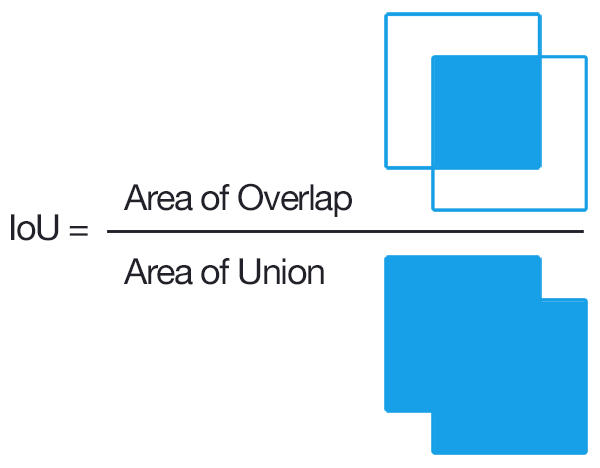
\includegraphics[width=6cm]{img/Intersection_over_Union_-_visual_equation.png}
    \caption[Visualization of Intersection over Union]{Visualization of Intersection over Union\\Source: Intersection over Union -- visual equation\protect\footnotemark{} by Adrian Rosebrock, CC BY-SA 4.0,\footnotemark{} via Wikimedia Commons}
    \label{fig:iou}
\end{figure}
\addtocounter{footnote}{-2}
\stepcounter{footnote}\footnotetext{\url{https://commons.wikimedia.org/wiki/File:Intersection_over_Union_-_visual_equation.png}}
\stepcounter{footnote}\footnotetext{\url{https://creativecommons.org/licenses/by-sa/4.0}}


\subsection{Trajectory Generation}

\label{ssec:trajectory_generation}

So far we worked with only two \glspl{det} at the same time and derived a set of conditions. In this section, we aim to make a use of a context of the whole \gls{ses}. We further show how we generate the actual trajectories.

Firstly, let us note that we can not apply the conditions from \autoref{ssec:nonspatial_merging} and \autoref{ssec:spatial_merging} to every pair of \glspl{det} for practical reasons. Comparing every \gls{det} with every other \gls{det} takes quadratic time with respect to number of \glspl{det} and for hundreds of thousands of \glspl{det} is unfeasible to compute on standard hardware. Therefore, we need to lower the number of comparisons.

In order to do so we leverage the way we use the timestamp as described in \autoref{ssec:nonspatial_merging}. We consider only \glspl{det} whose difference in timestamps are below a selected threshold. This means that we need to compare only pairs of \glspl{det} that fit within a selected ``sliding time window''. We process the \glspl{det} in order of their timestamp.

When we process a new \gls{det} we add it to the sliding window. At the same time we remove all the \glspl{det} from the sliding window that are older than the timestamp of the new detection minus the threshold. Then we compare the new \gls{det} with all the \glspl{det} within the window. Use of the sliding window dramatically decreases the number of comparisons needed.

However, this approach does not limit the length of the single trajectory by selected threshold. We use ``transitive'' information about the trajectory. Namely, if a \gls{det} ($A$) belongs to the same trajectory as \gls{det} ($B$) and \gls{det} ($B$) belongs to same trajectory as \gls{det} ($C$), we can conclude that the \gls{det} ($A$) and \gls{det} ($C$) is of the same trajectory.

This process of finding if there is a transitive link between the two \glspl{det} may also pose a limitation on the number of \glspl{det} we can process effectively. To improve the performance in this regard we use the standard Union-find architecture originally described by \cite{galler1964improved}. The architecture allows us to track which \glspl{det} belongs to which trajectory and merge them in almost constant\footnote{The actual complexity of the operation is inverse Ackermann function of the size of the structure per query (amortized) as was proved by \cite{tarjan1984worst}. For the details of the structure please refer to the attached code or the original research.} time per request.

Finally, let us note this approach of using transitive link is not only efficient but also has additional advantage. Let us consider a case where a person crosses entire view of a camera. Without this transitive connection we would need to set huge thresholds to match the first and last \gls{det} of this person (which would produce trajectories of poor quality). However, by using transitivity over other \glspl{det} we can match the first a last \gls{det} together ``through'' the \glspl{det} of the same person on the frames in between while keeping the thresholds low.

The overall approach for trajectory generation described in this subsection is summarized by \autoref{alg:trajectory_generation}.

\begin{algorithm}
 \SetKwData{Traj}{Trajectories}
 \SetKwData{Win}{SlidingWindow}
 \SetKwData{Det}{Detection}
 \SetKwData{ProcDet}{ProcessedDetection}
 \SetKwFunction{UnionFind}{UnionFind}
 \SetKwFunction{Queue}{Queue}
 \SetKwFunction{Top}{Top}
 \SetKwFunction{Ts}{Timestamp}
 \SetKwFunction{Pop}{Pop}
 \SetKwFunction{Add}{Add}
 \SetKwFunction{AddNs}{AddNewSet}
 \SetKwFunction{Union}{Union}
 \SetKwInOut{Input}{input}
 \SetKwInOut{Output}{output}

 \Input{List $X$ of detections sorted by timestamp, threshold $t$}
 \Output{List of generated trajectories (each trajectory as list of detections)}
 
 \BlankLine
 \Traj $\leftarrow$ \UnionFind{ }\;
 \Win $\leftarrow$ \Queue{ }\;
 \For{\Det $\in X$}{
  \While{\Det.\Ts $-$ \Win.\Top.\Ts $> t$} {
   \Win.\Pop{}\;
  }
  \Win.\Add{\Det}\;
  \Traj.\AddNs{\Det}\;
  \For{\ProcDet $\in$ \Win}{
   \If{All conditions for merging are met}{
    \Traj.\Union{\ProcDet, \Det}\;
   }
  }
 }
 \Return \Traj

 \caption{Trajectory Generation}
 \label{alg:trajectory_generation}
\end{algorithm}

\section{Identities}

\label{sec:generating_identities}

So far we have looked into how to cluster the \glspl{det} purely based on the metadata (i.e. how to create trajectories). Now we add the visual information (in form of feature vectors from \autoref{ch:features}) to also identify the same object in \glspl{det} that are physically far apart or captured by different cameras -- something that was not possible using just metadata. In other words we are interested in creating the \glspl{iden}. Each \gls{iden} then represents all the \glspl{det} of a single object. Finding the correct \glspl{iden} is the final goal of our algorithm, and of this thesis.

\subsection{Trajectory Merging}

The first approach we evaluate works with trajectories generated in the previous section. We consider trajectories as ``building blocks'' and merge them together into the \glspl{iden} by incorporating the visual information.

We base the merging of trajectories on the distance between the \glspl{det} (or more, precisely, corresponding feature vectors) from the trajectories. We explore multiple distance functions (Euclidean, Manhattan, Cosine -- for definitions please refer to \autoref{sec:distances}) and their effect on the quality of resulting \glspl{iden}.

The straight-forward approach would be to consider each pair of trajectories and to compare each \gls{det} from one trajectory to each \gls{det} from the other trajectory. If the distance between the corresponding feature vectors of any pair of \glspl{det} is lower than selected threshold, we merge the trajectories together. This is quite similar to merging \glspl{det} into trajectories as described in previous section. However, it shares the same disadvantage -- the total number of comparisons needed is quadratic in terms of number of \glspl{det}. In the case of trajectories we solved this problem by using sliding window. If we use the sliding window here we lose the ability to merge trajectories with significant ``time gaps''. Therefore, we show another approach to decrease the number of comparisons needed.


\subsubsection{Selection of Representants}

%We present a relatively simple approach to decrease number of comparison needed.

The idea behind this approach is to select from each trajectory a set of representants. We want to select a suitable set of representants that will preserve as much information as possible needed for creating appropriate \glspl{iden}. We then compare just pairs of representants instead of all pairs of \glspl{det}. As we show, if the representants are chosen well, the resulting \glspl{iden} will be nearly as good as if we were to compare all the pairs of \glspl{det}.

To show how to pick suitable representants, let us consider following case: let there be a trajectory and let us pick two \glspl{det} from the trajectory that are similar in terms of their feature vectors. Now consider additional trajectory and one arbitrary \gls{det} from this trajectory in particular. The situation is shown in \autoref{fig:triangular}. The question we focus on is whether we should merge these trajectories together based on the three selected \glspl{det} or not. The straight-forward way to do it would be to compare the \gls{det} from the second trajectory to both of the \glspl{det} from the first trajectory. Note due to the triangular inequality as the two \glspl{det} from the first trajectory are similar, the two computed distances from the third \gls{det} should be similar too. Therefore, if we make our decision regarding the merging the trajectories based on just one of the two distances, we (in most cases) make just as good decision as if we computed both distances. Note that this observation relies on the triangular inequality and therefore holds only if the distance function used is a metric.

\begin{figure}
    \centering
    \Large
    \def\svgwidth{\columnwidth}
    \scalebox{0.6}{\input{img/triangular.pdf_tex}}
    \caption[Usage of triangular inequality for the selection of representants]{Usage of the triangular inequality for the selection of representants. From the triangular inequality the distances $d_1$ and $d_2$ differ at most by the value of $d_s$, i.e. $\abs{d_1 - d_2} \leq d_s$}
    \label{fig:triangular}
\end{figure}

This leads us to the following idea: For each trajectory from each set of similar \gls{det} we set only one of them as a representant. To be more precise for each trajectory we set a set of representants such that for each \gls{det} within the trajectory there is at least one representant, for which the distance to the detection is at most some threshold $\Delta_{rep}$. Refer to \autoref{alg:representants} on how to select such representants.

\begin{algorithm}
 \SetKwInOut{Input}{input}
 \SetKwInOut{Output}{output}

 \Input{Trajectory $T$ (as a list of feature vectors of detections), Threshold $\Delta_{rep}$}
 \Output{List of feature vectors of representants}
 
 \BlankLine
 $R \leftarrow$ \emph{empty list}\;
 \For(\tcp*[h]{outer loop}){$D_{new} \in T$}{
  \For{$D_{rep} \in R$}{
   \If{$\delta(D_{new}, D_{rep}) \leq \Delta_{rep}$}{
    skip to the next iteration of outer loop\;
   }
  }
  append $D_{new}$ to $R$\;
 }
 \Return $R$
 \caption{Selection of representants of a trajectory}
 \label{alg:representants}
\end{algorithm}

In context of many trajectories and \glspl{det} this approach indeed gives some guarantees. To precisely show which, we firstly define a concept of well-separation:

\begin{defn}
\label{defn:well_sep}
We say that partitioning $A$ of set $D$ is well-separated by distance function $\delta: D \times D \goto \R_0^+$ with distances $\Delta_{within} \in \R_0^+$ and $\Delta_{between} \in \R^+$ if:
\begin{enumerate}[label=(\roman*)]
    \item $(\forall a, a' \in A) (\forall d \in a) (\forall d' \in a') (a \neq a' \Rightarrow \delta(d, d') > \Delta_{between})$ \label{item:between}
    \item $(\forall a \in A)(\forall d, d' \in a) (\exists n \in \N) (\exists (d_1, \ldots, d_n) \in a^n) (d = d_1 \land d' = d_n \land (\forall i) (\delta(d_i, d_{i+1}) \leq \Delta_{within}))$ \label{item:within}
\end{enumerate}
\end{defn}

The first condition requires different \glspl{iden} (partitions) to by far apart -- the distance between two closes \glspl{det} from different \glspl{iden} has to be at least $\Delta_{between}$. The other conidition on the other hand requires the \glspl{det} within a \gls{iden} to be close to each other. In particular for any two \glspl{det} from one \gls{iden} there has to be a path over the \glspl{det} from the \gls{iden} such that no two subsequent \glspl{det} are more than $\Delta_{within}$ apart.

Now consider a set of \glspl{det} and its partitioning (golden \glspl{iden}) and a metric function that separates the \glspl{iden} well with thresholds $\Delta_{within}$ and $\Delta_{between}$ s.t. $\Delta_{within} < \Delta_{between}$. Further assume that each \gls{iden} is partitioned into smaller trajectories (i.e. each trajectory contains \glspl{det} from only one \gls{iden}). It is easy to see that if we skip the representant selection and directly merge the trajectories (or in other words we pick all \glspl{det} as representants) which are closer than $\Delta_{mrg}$, s.t. $\Delta_{within} \leq \Delta_{mrg} \leq \Delta_{between}$ then we will obtain the original golden \glspl{iden}.

Now, let us select representants from the trajectories by \autoref{alg:representants} with threshold $\Delta_{rep}$. We show that if we select a threshold for merging trajectories a bit more precisely, we still obtain the golden \glspl{iden} even though we discard some of the \glspl{det} (and keep only the representants). It will turn out that the required threshold for merging needs to be between $\Delta_{within} + 2\Delta_{rep}$ and $\Delta_{between}$. Note that this claim holds only for metric functions as it requires triangle inequality. We formalize and then prove the claim:

% In context of many trajectories and detections this approach indeed gives some guarantees. Let us assume that we get a set of trajectories and we find set of representants by \autoref{alg:representants} with threshold $\Delta_{rep}$ for all trajectories. Given the representants of the trajectories, we merge the trajectories that have any pair of representants closer than merging threshold $\Delta_{mrg}$.

% If there is unknown partitioning (golden \glspl{iden}) that are ``well-separated'' in a certain sense by the distance function then we will obtain exactly this unknown golden partitioning. By the term ``well-separated'' we mean that the minimal distance between \glspl{det} from two distinct golden \glspl{iden} is at least $\Delta_{mrg}$ and that for each pair of \glspl{det} from the same golden \gls{iden} there exists path over \glspl{det} such that each subsequent \glspl{det} are at most $(\Delta_{mrg} - 2\Delta_{rep})$ apart. To visualize this situation see \autoref{fig:claim}. We formalize this claim:

\begin{figure}
    \centering
    \def\svgwidth{\columnwidth}
    \input{img/claim.pdf_tex}
    \caption[Visualization of claim \ref{clm:claim}]{Visualization of claim \ref{clm:claim}. The figure shows two \glspl{iden}, first of them divided into three trajectories, latter into two. Dots represent \glspl{det}, the black ones mark the representants. Solid lines (shown only is the first trajectory) connect \glspl{det} to the closest representant, these lines are at most $\Delta_{rep}$ long. Dashed lines connect representants themselves and thus are longer than $\Delta_{rep}$. Dotted lines connect \glspl{det} of different trajectories but the same \gls{iden} (only a few are shown). The gray lines connect \glspl{det} of different \glspl{iden}.
    
    The claim considers situation where all ``gray distances'' are at least $\Delta_{mrg}$ and where we can walk from any \gls{det} of one \gls{iden} to another \gls{det} from the same \gls{iden} only by using the lines that are at most $(\Delta_{mrg} - 2\Delta_{rep})$ long. In such cases the produced \glspl{iden} perfectly match the golden \glspl{iden} shown in the figure.}
    \label{fig:claim}
\end{figure}

\begin{claim}
\label{clm:claim}
Let:

\setlength{\itemsep}{0pt}
\setlength{\parskip}{0pt}

\begin{itemize}
    \item $D$ be a set of \glspl{det}
    \item $A$ a partitioning of $D$ (this represents golden \glspl{iden})
    \item $T$ partitioning of $D$ such that $(\forall t \in T) (\exists a \in A) (t \subseteq a)$ (this represents input ``clean'' trajectories)
    \item $\Delta_{rep}, \Delta_{mrg} \in \R^+$ such that $\Delta_{rep} < \Delta_{mrg}$
    \item $\delta$ be a metric function over $D$
    \item $r$ be a function $r: \Pt{D} \goto \Pt{D}$ such that $(\forall c \subseteq D)((r(c) \subseteq c) \land (\forall b \in c) (\exists b' \in r(c)) (\delta(b, b') \leq \Delta_{rep}))$ (this represents selection of representants obtained for example via \autoref{alg:representants})
    \item $\triangledown$ be a relation over $T$ such that $t\triangledown t' \Leftrightarrow (\exists d \in r(t)) (\exists d' \in r(t')) (\delta(d, d') \leq \Delta_{mrg})$ (two trajectories are in relation $\triangledown$ if we can merge them together)
    \item $\blacktriangledown$ be a transitive closure of $\triangledown$ (i.e. $t \blacktriangledown t' \Leftrightarrow (\exists n \in \N) (\exists (t_1, \ldots, t_n) \in T^n) (t = t_1 \land t' = t_n \land (\forall i) (t_i\triangledown t_{i+1}))$ (this relation is equivalence that represents final \glspl{iden} -- two trajectories are in relation $\blacktriangledown$ if and only if they were merged together)
\end{itemize}

If the partitioning $A$ is well separated by $\delta$ with distances $\Delta_{within} \leq (\Delta_{mrg} - 2\Delta_{rep})$ and $\Delta_{between} \geq \Delta_{mrg}$ then $t\blacktriangledown t' \Leftrightarrow (\exists a \in A) (t \cup t' \subseteq a)$ (i.e. produced \glspl{iden} exactly match golden \glspl{iden})

\end{claim}

\begin{myproof}
First, let us prove that $t \blacktriangledown t' \Rightarrow (\exists a \in A) (t \cup t' \subseteq a)$. We prove this by contradiction, i.e. we assume
that $t \blacktriangledown t'$ and $(\exists a \in A) (t \subseteq a)$ and $(\exists a' \in A) (t' \subseteq a')$ where $a \neq a'$. From property of $\blacktriangledown$ we know there is a sequence of $t_1, t_2, \ldots t_n$ (for some $n$), such that $(\forall i) (t_i \triangledown t_{i+1})$. Let
us take minimal $i$ such that $t_i$ and $t_{i+1}$ is not subset of the same
$a \in A$ (such $i$ exists as $t$ and $t'$ belong to different sets $a \in A$).
For such $i$ (since $t_i \triangledown t_{i+1}$) there is $d \in t_i$ and
$d' \in t_{i+1}$ such that $\delta(d, d') \leq \Delta_{mrg} \leq \Delta_{between}$. However since $d \in a$
and $d' \in a'$ (such that $a \neq a'$) this is in contradiction with \ref{item:between} of \autoref{defn:well_sep}.

Now, we prove that $(\exists a \in A) (t \cup t' \subseteq a) \Rightarrow t \blacktriangledown t'$. Let us choose $d \in t$ and $d' \in t'$ arbitrarily. By the
\ref{item:within} of \autoref{defn:well_sep} there is sequence $(d_1, \ldots, d_n) \in D^n$
such that $d = d_1 \land d' = d_n \land (\forall i) (\delta(d_i, d_{i+1}) \leq \Delta_{within} \leq \Delta_{mrg} - 2\Delta_{rep}$. Now we denote for each $i,$ $t_i \in T$ such that
$d_i \in t_i$. Finally, we denote $r_i = \mathrm{argmin}_{d' \in r(t_i)} \delta(d', d_i)$. If $t_i = t_{i+1}$ then $t_i \triangledown t_{i+1}$ by definition.
So let us consider cases where $t_i \neq t_{i+1}$. In such case we can bound
the distance between $r_i$ and $r_{i+1}$: We have $\delta(r_i, d_i) = \mathrm{min}_{d' \in r(t_i)} \delta(d', d_i) \leq \Delta_{rep}$ (where the last inequality holds from the properties of $r$). Similarly  $\delta(r_i, d_i) \leq \Delta_{rep}$. Finally we use triangle inequality to obtain: $\delta(r_i, r_{i+1}) \leq \delta(r_i, d_i) + \delta(d_i, d_{i+1}) + \delta(d_{i+1}, r_{i+1}) \leq \Delta_{rep} + (\Delta_{mrg} - 2\Delta_{rep}) + \Delta_{rep} = \Delta_{mrg}$. And as $r_i \in r(t_i)$ we can conclude that $(\forall i) (t_i \triangledown t_{i+1})$. Therefore $t \blacktriangledown t'$.\end{myproof}


\begin{cor}
If the distance between two closest \glspl{det} from different golden
\glspl{iden} is $\Delta_{between}$ and the distance between two most distant \glspl{det}
of the same golden \gls{iden} is $\Delta_{within} < \Delta_{between}$, then for any set of ``clean''
trajectories (i.e. if each trajectory contains \glspl{det} only from single
golden \gls{iden}) the \autoref{alg:representants} for representant selection
with threshold $\Delta_{rep} < (\Delta_{between} - \Delta_{within}) / 2$ followed by merging based on representants with
threshold $\Delta_{mrg}$ s.t. $\Delta_{within} \leq \Delta_{mrg} < \Delta_{between}$ produces the golden \glspl{iden}.
\end{cor}

Even thought we can not be sure that the preconditions of the corollary hold for our practical application, we see this as a theoretical justification for our approach of selecting representants. 

%Furthermore, we evaluate this approach even for the cosine distance function, which is not a metric function.

% Let us note that the original assumption of the corollary is fulfilled if the Triplet Loss
% over the examinated dataset is zero (and in some cases even if it is positive).
% This is usually too strong assumption to make, however it still gives us some
% theoretical justification for our approach.

% In case that $\delta$ is not metric function but just a generic distance
% function we have no such guarantees. However, we still evaluate this approach
% even for such distance functions.

\subsection{Direct Identity Generation}

We have presented two-step approach for the identity generation. In the first step we generate
trajectories and during the second step we merge these trajectories into
the \glspl{iden}.

However, we also experiment with the approach where we generate the identities directly from the \glspl{det} (and omit the trajectories). This approach would work similarly to the original trajectory generation (from \autoref{ssec:trajectory_generation}) where we have a sliding window of \glspl{det} and we merge two sets of \glspl{det} together if we find two similar \glspl{det}. This approach has significant drawback of not being able to merge two sets of \glspl{det} together if there is too big ``time gap'' between two consecutive \glspl{det}. Nevertheless, we believe it is worth to experiment with this direct approach.

However, we still want to be able to assign two \glspl{det} to the
same \gls{iden} at least if they both fit into the sliding window and are from different cameras. Therefore, our approach will be as follows: If we are
considering two \glspl{det} for merging, we evaluate the spatial information
exactly as in \autoref{ssec:spatial_merging}. If all the conditions are met,
we merge the corresponding set of \glspl{det}. If one of the thresholds is
exceeded, then we evaluate the visual information. If the corresponding feature
vectors are closer than the pre-selected threshold, we merge the corresponding set \glspl{det} even though the information from metadata is not conclusive.

\section{Summary}

This chapter elaborated on two ways to generate \glspl{iden} -- trajectory generation with subsequent merging and direct approach. Both are dependent on the choice of the feature vectors (which we described in \autoref{ch:features}). Furthermore, each approach is dependent on the selection of additional hyper-parameters (such as thresholds). In \autoref{ch:evaluation} we aim to find suitable hyper-parameters by empirical testing. We summarize the parameters we search for suitable values of:

\begin{itemize}
    \item Size of the sliding window
    \item Threshold for displacement of \glspl{det}
    \item Threshold for relative displacement
    \item Threshold for Intersection over Union
    \item Distance function
    \item Threshold for distance over feature vectors
\end{itemize}
\chapter{Evaluation}

%123456789 123456789 123456789 123456789 123456789 123456789 123456789 123456789

\label{ch:evaluation}

In this chapter we aim to empirically evaluate the approaches we have described
in previous chapters of this work.

\section{Datasets}

\label{sec:datasets}

In this thesis we work with two distinct \glspl{ses}. In particular work with the \glspl{det} of people only as they are the main focus of this work and other classes are not well represented in our dataset.

The first \gls{ses} comes from processing recording of single camera which captured a public square. The original recording is about 5 minutes long. The total number of \glspl{det} extracted from the recording is 181,792. We only keep \glspl{det} of people, furthermore we discarded all the ``faulty'' \glspl{det} such as \glspl{det} of shadows, trees, or when there were multiple \glspl{det} of the same person in a single frame. Overall we have left in this \gls{ses} 71,732 \glspl{det}, which we manually sorted into 274 different \glspl{det}. The main usage of this \gls{det} is to be a training dataset for training neural network based approaches to extract feature vectors from the images of \glspl{det}. The manual annotation serves as a golden truth for this training. A frame from this \gls{ses} and extracted \glspl{det} can be seen in \autoref{fig:single_session}.

\begin{figure}
    \centering
    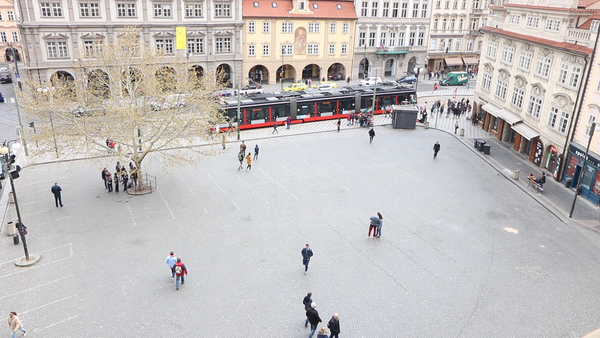
\includegraphics[width=0.48\textwidth]{img/frame_single_session_smaller.png}
    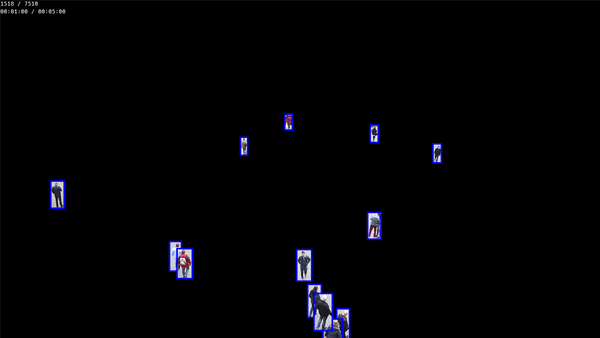
\includegraphics[width=0.48\textwidth]{img/frame_single_session_det_smaller.png}
    \caption{Frame from first session and extracted detections}
    \label{fig:single_session}
\end{figure}

We use the second \gls{ses} for actual evaluation of tested approaches. This second session is constructed from the recording of two simultaneously recording camera. The recording is over two minutes long. The view of the cameras partially overlap. In this session total of 147,681 \glspl{det} were extracted. Just as in case of the previous \gls{ses}, we filter some \glspl{det} out as not usable. There are 15,757 \glspl{det} remaining. The lower ratio of usable \glspl{det} compared to the previous case was cased mainly by many ``faulty'' \glspl{det} of statues and lamps which were not presented in the view for the first \gls{ses}. We sorted these \glspl{det} into 52 unique \glspl{iden}. These \glspl{iden} were used as a ground truth for actual evaluation of our approach. Examples of frames from this \gls{ses} is in \autoref{fig:double_session}.

\begin{figure}
    \centering
    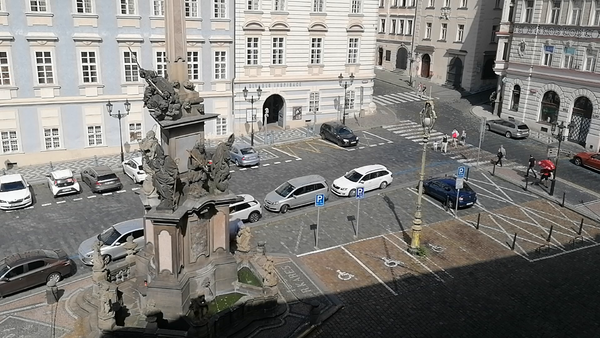
\includegraphics[width=0.48\textwidth]{img/frame_double_session_1_smaller.png}
    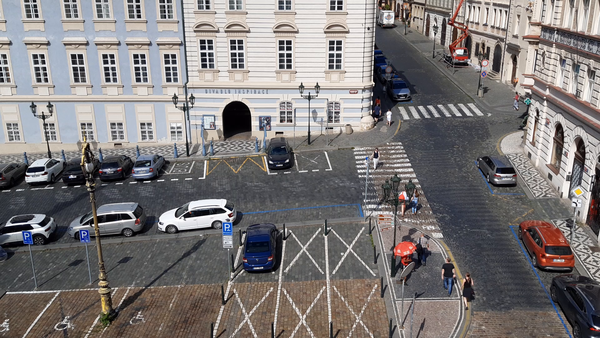
\includegraphics[width=0.48\textwidth]{img/frame_double_session_2_smaller.png}
    \caption{Frames from second session}
    \label{fig:double_session}
\end{figure}

The recordings for those two \glspl{ses} are entirely disconnected -- they
capture entirely different place and were recorded at different time. That gives
us unbiased estimation of the quality of our algorithm in terms of
\autoref{eq:mla}. It would be better to evaluate our algorithm to multiple
\glspl{ses}, however due to technical difficulty of creating new \gls{ses}
(especially in terms of annotating the data), we leave more thorough evaluation
to feature work.

\section{Feature vectors}

As the first step of actual evaluation of our approaches we evaluate the
quality of feature vectors as described in \autoref{ch:features}. We shall
evaluate this part purely based on how well the resulting feature vectors
separate the golden \glspl{iden} from each other. We recognize there is some
information lost, as we skip the final step in this evaluation -- that is to
construct actual \glspl{iden} and compare them with the golden \glspl{iden}.
However, this preliminary evaluation is computationally less expensive and
therefore we may experiment with broader spectrum of parameters. We shall
select couple of best performing setting and verify its usefulness in later
stages.

\subsection{Measures of Quality}

This preliminary testing offer simpler statistics for evaluation. In this scenario we need to just look into distances between \glspl{det} of the same golden \gls{iden} and the distances between \glspl{det} of distinct golden \glspl{iden}. We can further associate each approach with a threshold. The ideal scenario would be that the maximal distance between \glspl{det} from the same \gls{iden} would be at most this threshold and all the distances between \glspl{det} from distinct \glspl{iden} would be greater than the threshold. However, in most cases we do not have such ideal classifier. Thus we often need to deal with misclassified samples.

Overall we can assign every pair of detection in on of four standard categories. First two are \glspl{tp} and \glspl{tn} they represent correct classification -- pair of \glspl{det} from the same \gls{iden} with distance between them below selected threshold and pair of \glspl{det} from distinct \glspl{iden} with distance over the threshold respectively. The other categories are \glspl{fp} -- pairs that are of different \glspl{iden} but with distance below the threshold -- and \glspl{fn}, that are pairs of \glspl{det} from the same \gls{iden} but with the distance over the threshold.

This notation allows us to introduce two standard derived quantities --- \gls{tpr} and \gls{fpr}:

\begin{align*}
    \mathrm{TPR} &= \frac{\mathrm{TP}}{\mathrm{TP} + \mathrm{FN}} \\
    \mathrm{FPR} &= \frac{\mathrm{FP}}{\mathrm{FP} + \mathrm{TN}}
\end{align*}

Notice that when we increase the threshold, increase the number \glspl{tp} and \glspl{fp} and decrease number of \glspl{tn} and \glspl{fn}. In terms of rates, that means that both \gls{tpr} and \gls{fpr} increases. This allows us to draw a plot of how \gls{tpr} depends on \gls{fpr}. That is a quite common way to elaborate on the quality of \gls{ml} algorithm. The resulting plot is often called \gls{roc} curve.

Ideal classifiers would have a \gls{roc} curve going through a point
(0, 1). Such classifier with corresponding threshold would correctly
classify every input, positive or negative. We usually do not
have access to ideal classifiers. In such case we are, broadly speaking,
want to come up with classifier that have \gls{roc} curve as close to
point (0, 1) as possible.

However, \gls{roc} curves gives us more in-depth view into the classifier.
The curve shows which trade-offs between \glspl{fp} and \glspl{fn} (or in terms
of the axis \gls{fpr} and \gls{tpr}) are possible for given classifiers.

While the \gls{roc} curve offers quite useful evaluation of the
selected approach, it is often useful to express the quality of the
approach as a single number. Some information will be lost this way,
on the other hand it offers very straight-forward way to compare different
classifiers. For this evaluation we leverage also leverage the \gls{roc} curve.
In particular we compute the area under the curve. Generally, the greater
the area the better classifier we have.

Finally, let us note that we want to get feature vectors that help us to find the same object in physically distant \glspl{det}. Therefore, we are not really interested in the distance between \glspl{det} of the same \gls{iden} from subsequent frames (as they would be matched by metadata anyways without the visual information). Therefore, for this preliminary evaluation (and drawn \gls{roc} curves) out of all ``positive'' pairs (i.e. pairs of \glspl{det} from the same \gls{iden}) only those which are either from different cameras or are at least 2 seconds apart.

\subsection{Evaluation of Color Histograms}

Firstly, we aim to evaluate various approaches for feature vector generation
based on the color histograms. To recapitulate there are several basic choices
for histogram generation we need to evaluate (please refer to
\autoref{sec:histograms} for detailed explanation):

\begin{itemize}
    \item Selection of color model
    \item Type of background filtering
    \item Number of bins of a histogram
    \item Choice of distance function
\end{itemize}

\subsubsection{Evaluation of Background Filtering}

As there are too many options per category to evaluate all combinations we
firstly evaluate which background filtering mechanism works best for us. As we
aim to decide what section of the crop is important for the re-identification
the selection of background filtering should be relatively independent of
the choice of color model and number of bins. For the experiments in this
subsection we selected a hue and saturation with histogram with 8 bins in
each component (i.e. 64 bins total).

Let us recall that we reviewed several approaches to background filtering.
Each approach allows for fine-tuning via various parameters:

\begin{itemize}
    \item No background filtering -- no additional parameters
    \item Filtering using cropping -- total of three parameters: percentage of the image cropped from left and right, percentage of the image cropped from the bottom, and percentage of the image cropped from the top
    \item Weighting by Gaussian -- total of two parameters: center of the Gaussian along $y$-axis and the scale of the Gaussian
\end{itemize}

For each of these approaches we use grid search to find optimal values of
these parameters. The main value we use for comparison is the size of the
area under the \gls{roc} curve. However, we still explore some of the
\gls{roc} curves directly.

\begin{figure}
    \centering
    \def\svgwidth{\columnwidth}
    \Large
    \scalebox{0.6}{\input{img/aoc_crop_30.pdf_tex}}
    \scalebox{0.6}{\input{img/aoc_crop_20.pdf_tex}}
    \scalebox{0.6}{\input{img/aoc_crop_40.pdf_tex}}
    \caption{Area under the ROC curve for various copping setting}
    \label{fig:aoc_crop}
\end{figure}

As we can see from the measurements in \autoref{fig:aoc_crop} any method of background filtering significantly improved the quality of the feature vectors. We note that we achieved the best performance with cropping when we 
cropped 30\% image from the left and right side, 20\% from the top and 30\%
from the bottom (although variant with 20\% achieved almost as good results). An example of such cropping can be seen in
\autoref{fig:best_cropping}.

\begin{figure}
    \centering
    \includegraphics{img/0.png} \includegraphics{img/1.png} \\
    \includegraphics{img/0_crop.png} \includegraphics{img/1_crop.png}
    \caption{Example of most effective cropping}
    \label{fig:best_cropping}
\end{figure}

\begin{figure}
    \centering
    \def\svgwidth{\columnwidth}
    \Large
    \scalebox{0.6}{\input{img/aoc_gauss.pdf_tex}}
    \caption{Area under the ROC curve for various setting of Gaussian weighting}
    \label{fig:aoc_gauss}
\end{figure}

In terms of weighting with Gaussian, we have achieved the best results
by offsetting the Gaussian slightly above the center of the image, to 40\%
of the height of the image to be precise. The best setting for the scale
of the Gaussian seems to be 0.2 or 0.1 of the dimensions of the image. For detailed results
of the grid search see \autoref{fig:aoc_gauss}.

As we can see in \autoref{fig:roc_background} all the selected approaches
with background filtering gives almost identical results.

\begin{figure}[tb]
    \centering
    \def\svgwidth{\columnwidth}
    \input{img/background_roc.pdf_tex}
    \caption{ROC curve of various type of background filtering}
    \label{fig:roc_background}
\end{figure}

\subsubsection{Choice of distance function}

Another subject of our experiments is the choice of distance function. In
\autoref{ssec:used_distances} we introduced three distance functions --
Euclidean, Manhattan and cosine. As we can see in \autoref{fig:roc_distances}
the choice of distance function have significant effect on the results.
The worst distance function seems to be Euclidean distance. The best one,
especially while preserving lower \gls{fpr} seem to be Manhattan distance.
After all, Manhattan distance has quite straigh-forward explanation in context
of histograms -- it is simple the amount each bin needs to decrease or increase
in order to achieve the second histogram.

\begin{figure}
    \centering
    \def\svgwidth{\columnwidth}
    \input{img/roc_distances.pdf_tex}
    \caption{ROC curve of various distance functions}
    \label{fig:roc_distances}
\end{figure}

\subsubsection{Selection of Color Model and Number of Bins}

The last parameter we need to appropriately set is the actual color model
and number of bins per histogram. We explore several color models:

\begin{itemize}
    \item RGB model
    \item HSV model (we select hue component for one histogram and both hue and saturation component for another one)
    \item YUV model (we select UV components)
\end{itemize}

\begin{figure}
    \centering
    \def\svgwidth{\columnwidth}
    \Large
    \scalebox{0.7}{\input{img/model_bins.pdf_tex}}
    \caption[Area under the ROC curve for various color models and number of bins]{Area under the \gls{roc} curve for various color models and number of bins. Number of bins are displayer per channel. Total number of bins for HS and UV is number of bins per channel squared and for RGB it is number of bins per channel cubed. For some combinations were not explored as a total number of bins for these combination requires too much memory stored per each feature vector.}
    \label{fig:model_bins}
\end{figure}

For each model we explore various numbers of bins. The sizes of areas under the corresponding \gls{roc} curves is displayed in \autoref{fig:model_bins}. Contrary to our original
assumption the results gives usage of the raw RGB channels. The best variation in particular was with 4 bins per channel (i.e. 64 bins total).

This can be explained by various phenomena For one the varying lightning
conditions are not as common in our dataset as we expected. The other aspect
is that as we notice large quantity of the images are of people with black or
dark clothing. The downside of using hue as a component in histograms is that
hue can change very significantly case of black and white colors even in small
changes in actual color. See \autoref{fig:bad_hue} for the visualization.

\begin{figure}
    \centering
    \includegraphics[width=3cm]{img/bad_hue_orig.png}
    \includegraphics[width=3cm]{img/bad_hue_hue.png}
    \caption[Hue extraction from an image]{Hue extraction from an image. The image on the left is original. The right image was obtained by preserving hue of each pixel but setting saturation and value to the same high level. As we can see, the mono-colored black coat has various hue levels and on the other hand the black coat and the white background is represented by similar hue levels even tough both are of entirely different colors.}
    \label{fig:bad_hue}
\end{figure}

We aim to support this reasoning by considering pixels with low ($< 0.2$)
value as black and non-black pixels with low saturation ($< 0.2$) as white and
assign them to separate bins. As we can see in \autoref{fig:black_white_roc} this indeed
significantly improved the feature vector. However it still seems best to use basic RGB decomposition.

\begin{figure}
    \centering
    \def\svgwidth{\columnwidth}
    \input{img/black_white_roc.pdf_tex}
    \caption[Effect of adding black and white bins to hue histograms]{Effect of adding black and white bins to hue histograms. The figure shows \gls{roc} curves of histogram based approaches of with RGB, hue \& saturation and only hue decomposition with the best performing number of bins in each category. The plot shows improved performance obtained by adding black and white bins to the latter two categories.}
    \label{fig:black_white_roc}
\end{figure}

\subsection{Evaluation of Deep Learning Approaches}

In the previous section we have focused on the feature vectors drawn using
histograms. Now, we explore the approaches involving \glspl{nn}. In this
section we make use of pre-trained model in Tensorflow framework
(\cite{tensorflow}) and described in \autoref{sec:existing_architectures}.

\subsubsection{Direct Use of Pre-trained Models}

Perhaps the simplest usage of pre-trained models is to use them directly
without any additional training. The potential in such usage is that the
second to last layer (i.e. prior actual ``classification'' layer) has to
contain enough of information to classify the original image. Therefore,
we experiment whether such information is enough for our purposes.

As we already stated, we mainly use ResNet and MobileNet architectures
pre-trained on the ImageNet dataset. These archtecture, as is common,
requires the input of the fixed size. That means we need to rescale all the
input images. As the sizes of original bounding boxes are diverse (see
\autoref{fig:size_dist}, we can not avoid distorting the original images.
Therefore, we evaluate performance of the network with various input sizes.

\begin{figure}
    \centering
    \def\svgwidth{\columnwidth}
    \input{img/size_distribution.pdf_tex}
    \caption{Distribution of heights and widths of detections}
    \label{fig:size_dist}
\end{figure}

The \gls{roc} curves (with the same setting as in previous subsection) of the
annotation with the pre-trained models in \autoref{fig:pretrained_nn_roc}.
We have evaluated various input sizes. In case of MobileNet we have tested
all the input sizes that are available for the architecture. As for the 
ResNet we have tested lower number of smaller sizes, mainly for its higher
complexity and poorer performace compared to the MobileNet.

As we can see directly from the \gls{roc} curves, the decidedly best setting for this type of the \gls{nn} annotation is MobileNet with input resized to $128 \times 128$. 

\begin{figure}
    \centering
    \def\svgwidth{\columnwidth}
    \input{img/pretrained_nn_roc.pdf_tex}
    \caption{ROC curves of pre-trained model}
    \label{fig:pretrained_nn_roc}
\end{figure}

We have also experimented with different distance functions. As you can in \autoref{fig:basic_nn_roc_dist} the effect of different distance functions are rather small. Especially between Euclidean and Manhattan distance.

\begin{figure}
    \centering
    \def\svgwidth{\columnwidth}
    \input{img/basic_nn_roc_dist.pdf_tex}
    \caption{Comparison of effect of different distance functions on MobileNet with shape 128}
    \label{fig:basic_nn_roc_dist}
\end{figure}

\subsubsection{Fine-tuning the Pre-trained Models}

As we showed we achieved somewhat useful results with just using as-is pre-trained models. However such models were trained for classification tasks and therefore there should be a room for improvement when trained specifically on \reid{} task. For this reason we aim to train the networks (with weights initialized as trained on classification task) on our dataset.

For the first experiment in this regard we do not change the architecture at all. We just use the architecture as-is and train in on our dataset using Triplet Loss (\autoref{sec:triplet_loss}).

\begin{figure}
    \centering
    \def\svgwidth{\columnwidth}
    \large
    \scalebox{0.8}{\input{img/training_loss.pdf_tex}}
    \caption{Training loss during training}
    \label{fig:training_loss}
\end{figure}

As we can see from the log in \autoref{fig:training_loss} we significantly reduce the training error by this approach. However when we tried to apply the resulting \gls{nn} on our testing \gls{ses} (see \gls{roc} curve in \autoref{fig:basic_nn_overfit_roc}), we see that the performance of the network significantly decreased. Furthermore, we can see that the performance worsen even after the single epoch of training. The weights are being altered too much even in single epoch as the original capabilities of the network is lost.

\begin{figure}
    \centering
    \def\svgwidth{\columnwidth}
    \input{img/basic_nn_overfit_roc.pdf_tex}
    \caption{Performance of the network after training for several epochs}
    \label{fig:basic_nn_overfit_roc}
\end{figure}

We therefore lowered the learning rate to try to preserve the original information within the network. This proved to be the correct approach as we managed to significantly increase the performance of the network as you can see in \autoref{fig:basic_nn_lr1_roc} and \autoref{fig:basic_nn_lr2_roc}.

\begin{figure}
    \centering
    \def\svgwidth{\columnwidth}
    \input{img/basic_nn_lr1_roc.pdf_tex}
    \caption{Performance of the network after training with learning rate 0.0001}
    \label{fig:basic_nn_lr1_roc}
\end{figure}

\begin{figure}
    \centering
    \def\svgwidth{\columnwidth}
    \input{img/basic_nn_lr2_roc.pdf_tex}
    \caption{Performance of the network after training with learning rate 0.00002}
    \label{fig:basic_nn_lr2_roc}
\end{figure}

Now, we proceed evaluate effect of different distance functions. This also means to train a new \gls{nn} as used loss function (Triplet Loss -- \autoref{eq:triplet}) depends on the choice of the distance function. In other related work we see the Triplet Loss used either with Euclidean distance or Cosine distance (or alternatively squared Euclidean distance\footnote{As the final layer of our \glspl{nn} is normalizing layer, the square Euclidean distance and cosine distance are proportional to each other: $\delta_{euclid}(\vec{x}, \vec{y}) = 2 - 2\vec{x}^T\vec{y} = 2 - 2 \cos(\vec{x}, \vec{y})$ (as the norms of input vectors are 1).}). However, we also aim to verify usefulness of Manhattan distance, as it works well with the histogram approach.

\begin{figure}
    \centering
    \large
    \def\svgwidth{\columnwidth}
    \scalebox{0.8}{\input{img/lr_heatmap_cosine.pdf_tex}}
    \vspace{1cm}
    
    \def\svgwidth{\columnwidth}
    \scalebox{0.8}{\input{img/lr_heatmap_manhattan.pdf_tex}}
    \caption{Area under the ROC curve for various learning rates and distances}
    \label{fig:lr_heatmap}
\end{figure}

As you can see in \autoref{fig:lr_heatmap}, the with different distance functions (both cosine and Manhattan) we achieved better results. However we can notice that even with lowered learning rate the best results on terms of area under the \gls{roc} curve are achieved by network trained only for single epoch. Therefore, we split each epoch and instead of using all 71,732 \glspl{det} in each epoch, we use only 640 \glspl{det} split among 32 batches per epoch.

As we can see the area under the \gls{roc} curve increases during the several initial epochs. In case of cosine distance, it reaches maximum around the 40\textsuperscript{th} epoch with value 0.9145. See the plot in \autoref{fig:mini_epoch_cos}. With Manhattan distance the maximum was reached very early and probably could be improved by further testing. However, since we achieve better results with cosine distance, we do not evaluate the Manhattan distance approach any further.

\begin{figure}
    \centering
    \def\svgwidth{\columnwidth}
    \input{img/mini_epoch_cos.pdf_tex}
    \caption{Area under the ROC curve with smaller epoch}
    \label{fig:mini_epoch_cos}
\end{figure}

We also explored the effect of using Semihard instead of Hard Triplet Loss. The model trained slightly faster with the Semihard Loss. It achieved the best performance so far. However, compared the Hard loss, this increase in performance is barely noticeable. The best value of area under the curve is 0.9161. You can see the comparison during the training in \autoref{fig:semi_hard_loss}.

\begin{figure}
    \centering
    \def\svgwidth{\columnwidth}
    \input{img/semi_hard_loss.pdf_tex}
    \caption{Area under the ROC curve while using Hard and Semihard loss}
    \label{fig:semi_hard_loss}
\end{figure}

\subsubsection{Altering the architecture}

So far we focused on finding suitable hyperparameters but we do not change the structure of the MobileNet itself, aside from the removal of last ``classification'' layer. Now, we briefly investigate if we can improve our model by if slightly altering the architecture could improve the performance of the network. Based on findings in the this section so far we use the semihard loss with cosine distance.

The alteration we use is to add a dense layer at the end of the network. This is motivated by the fact that we removed the last layer (originally trained by softmax). By this removal the network could lose some of its capabilities. By adding another similar layer the netwourk could retrieve some if its potentially lost ability. 

To keep things simple, we keep the size of the new layer same as the layer before it, that is 1280 neurons. We also experiment if ``freezing'' (i.e. not changing the weights of the original MobileNet weights during training) helps.

As it turned out, the setting where we trained the MobileNet with added dense layer without freezing indeed produced the best model so far. That being said the difference in the area under the \gls{roc} is negligible -- we achieved area of 0.9192. You can compare the actual \gls{roc} curve of this model and two models without dense layer in \autoref{fig:final_roc}. As you can see in the plot, the performance of the network with the dense layer is worse in very low level of \gls{fpr} (approx. below 0.1), while noticeably better for higher values of \gls{fpr}. We evaluate both networks (with and without added dense layer) in the next step of creating \glspl{iden}.


\begin{figure}
    \centering
    \def\svgwidth{\columnwidth}
    \input{img/final_roc.pdf_tex}
    \caption{ROC curves of final approaches for feature extraction}
    \label{fig:final_roc}
\end{figure}

These results were achieved by using MobileNet as pre-trained on ImageNet dataset with replaced last layer. We also experimented with using weights that we learned during the training without the added dense layer. We added the dense layer to the network and continue with the trainig with the added layer. However we did not manage to produce improved results. 

\section{Trajectory Construction}

We now briefly remind the reader of the next step which is trajectory construction. Unlike in case of feature vectors we do not conduct thorough evaluation of various approaches, as the desired result of this step is strongly influenced by the next step which is actual \gls{iden} construction.

Nevertheless, we at least suggest some useful threshold for the suggested quantities as described in \autoref{ssec:spatial_merging} -- displacement, relative displacement and Intersection over Union. We can draw suitable thresholds directly from the training set. Note that the threshold should be set in a such manner that each resulting trajectory should contain \glspl{det} only from one \gls{iden}, as we merge the trajectories but never split them afterwards. If we have a trajectory which contains \glspl{det} from two or more different golden \glspl{iden} we can never fix this ``impurity''.

This leads us to simple way to suggest suitable thresholds. For now let us consider simple displacement. We analyzed the training dataset. In the dataset we looked into each pair of the \glspl{det} which are no more than 0.2 seconds from each other and they are from different golden \glspl{iden}. For each such pair we recorded the displacement and consider the value as ``negative sample''. To obtain ``positive samples'' we processed all the \glspl{iden} in order of their timestamps. For any subsequent pair of \glspl{det} in each trajectory, if the pair is less the 0.2 seconds apart, we consider the corresponding value of displacement as ``positive sample''.

Then we computed the minimum over the negative samples (which gives us suitable starting point of which value to use on the testing dataset). Furthermore we counted how many positive samples are greater than the computed minimum (which gave us rough estimation of how quality the quantity is).

\begin{table}[]
    \centering
    \begin{tabular}{c|r|r}
         Quantity & Threshold & False over threshold  \\ \hline
         Displacement & 5.385 & 1.2938\% \\
         Relative Displacement & 0.037 & 0.4959\% \\
         Intersection over Union & 0.733 & 0.4636\%
    \end{tabular}
    \caption{Comparison of metadata quantities on training session}
    \label{tab:metadata_comparison}
\end{table}

We did this analysis for each of the considered quantities. The results are recorded in \autoref{tab:metadata_comparison}. As we can see the basic displacement has relatively low usefulness as the ratio of the positive samples above the threshold is relatively low. We shall consider the remaining two -- relative displacement and Intersection over Union in further steps.

\section{Identity Construction}

In this section we review the final results of our algorithm. 
\chapter{Implementation}

The goal of this chapter is to summarize the architecture of the underlying implementation and general design. For the detailed guide on how to use it for \gls{iden} generation on a new data please read \autoref{ch:guide}. For the implementation details, please refer to attached code.

As we mentioned in the \autoref{sec:vl}, whole our work is designed as a module for \gls{VL}. Even though our work is largely independent of other modules within the framework of \gls{VL}, it shares one main component and that is the relation database. We use the database as an \gls{api} for communication for other modules as well as a place to store our intermediate results.

In our implementation we used and tested usage of PostgreSQL as an management system. However, as we use SQLAlchemy library (\cite{sqlalchemy}) for all the communication with the database, so usage of another management system should be without any problems.

Overall, the implementation is split into a few parts. Each part processes the input from the database and writes there also the results. The primary purpose of each part is to be used as a python module. However, for the purposes of testing and simple evaluation, we also add an command line interface for each part.

One of the parts is responsible for creating feature vectors described in \autoref{ch:features}. For the histogram approaches the process is straight-forward. The \glspl{det} from the selected cameras are querried, the histograms computed and then commited back to the database. For the approaches involving annotation with neural network we can supply the network externally, in such case the process is similar. We also have an option to train the network on the data in the database. In such case the training data are first retrieved, then the network is trained and stored locally for subsequent usages. After the network is trained the data for annotation is annotated using the network and the feature vectors are again committed into the database.

The other part is responsible for clustering the \glspl{det} (\autoref{ch:iden_construction}), that is for both -- trajectory generation and identity generation. For this process the \glspl{det} form given cameras are again retrieved from the database along, if applicable, with the corresponding feature vectors created with the selected settings. If we use the constriction of trajectories from before they are also queried. Once the \glspl{det} are clustered according to the parameters, the resulting trajectories or \glspl{iden} are again commited to the database for processing via other \gls{VL} modules.

We also provide a tool for manual annotation of the \glspl{det} that we used for obtaining the ground truth used for the experiments. The tool queries the \glspl{det} from the database as well as selected \glspl{iden} or trajectory. User then can see the the \glspl{det} frame-by-frame as well as their division to \glspl{iden}. It is possible to re-assign the wrongly assigned \glspl{det} to different \gls{iden}. This approach allows for semi-automated anno
\chapter*{Conclusion}
\addcontentsline{toc}{chapter}{Conclusion}


%%% Bibliography
%%% Bibliography (literature used as a source)
%%%
%%% We employ bibTeX to construct the bibliography. It processes
%%% citations in the text (e.g., the \cite{...} macro) and looks up
%%% relevant entries in the bibliography.bib file.
%%%
%%% The \bibliographystyle command selects, which style will be used
%%% for references from the text. The argument in curly brackets is
%%% the name of the corresponding style file (*.bst). Both styles
%%% mentioned in this template are included in LaTeX distributions.

\bibliographystyle{plainnat}    %% Author (year)
% \bibliographystyle{unsrt}     %% [number]

\renewcommand{\bibname}{Bibliography}

%%% Generate the bibliography. Beware that if you cited no works,
%%% the empty list will be omitted completely.

\bibliography{bibliography}

%%% If case you prefer to write the bibliography manually (without bibTeX),
%%% you can use the following. Please follow the ISO 690 standard and
%%% citation conventions of your field of research.

% \begin{thebibliography}{99}
%
% \bibitem{lamport94}
%   {\sc Lamport,} Leslie.
%   \emph{\LaTeX: A Document Preparation System}.
%   2nd edition.
%   Massachusetts: Addison Wesley, 1994.
%   ISBN 0-201-52983-1.
%
% \end{thebibliography}


%%% Figures used in the thesis (consider if this is needed)
\listoffigures

%%% Tables used in the thesis (consider if this is needed)
%%% In mathematical theses, it could be better to move the list of tables to the beginning of the thesis.
\listoftables

%%% Abbreviations used in the thesis, if any, including their explanation
%%% In mathematical theses, it could be better to move the list of abbreviations to the beginning of the thesis.
%\chapwithtoc{List of Abbreviations}

\clearpage
\printnoidxglossaries

%%% Attachments to the master thesis, if any. Each attachment must be
%%% referred to at least once from the text of the thesis. Attachments
%%% are numbered.
%%%
%%% The printed version should preferably contain attachments, which can be
%%% read (additional tables and charts, supplementary text, examples of
%%% program output, etc.). The electronic version is more suited for attachments
%%% which will likely be used in an electronic form rather than read (program
%%% source code, data files, interactive charts, etc.). Electronic attachments
%%% should be uploaded to SIS and optionally also included in the thesis on a~CD/DVD.
%%% Allowed file formats are specified in provision of the rector no. 72/2017.
\appendix
\chapter{User Guide}
%\chapter{Attachments}
%
%\section{First Attachment}

\clearpage
\listoftodos

\openright
\end{document}
